\chapter{Feature Engineering}
\label{ch:feature_engineering}
The ultimate goal of Feature Engineering is to clean the data and transform the
data with heuristic strategies that tag events coming from signal sources, as
separate from events which come from our background, so that we can proceed with
the calculation of the physics asymmetry.

Even with the Forward Upgrade (Section~\ref{sec:forward_upgrade}), our data set
is still composed mostly of background events
(Figure~\ref{fig:data_composition}). The primary constituents of the data set
are muons from the following sources:

\begin{itemize}
  \item \textbf{Hadronic Background}
    \begin{itemize}
      \item The hadronic background is composed of hadrons which are produced
        from the primary event vertex, and then travel into the muon arms. The
        hadrons then decay in the muon arms, and create hits at each station,
        which are mis-reconstructed as high-$p_T$ muons.
    \end{itemize}
  \item \textbf{Muon Background}
    \begin{itemize}
        \item The muon background is composed of processes which produce real
          muons which fall into a similar kinematic regime of the W-genic muons
    \end{itemize}
  \item \textbf{W Signal}
    \begin{itemize}
        \item These are muons we are looking for. They come from the W boson
          decay, and carry information about the proton spin.
    \end{itemize}
\end{itemize}

We will differentiate these types of data in two different step. In the first
step, we will use likelihood event selection, where we lump hadronic background
and muon background together, and merely distinguish it from W-genic events. In
the second stage, we will further differentiate our model for the background,
drawing heavily on the data to understand the hadronic background, and providing
simulations of the W-genic events as well as simulation cocktail for other muon
background events. Before we discuss this differentiation, it is important to
discuss the simulations, as the rest of the analysis hinges on the simulation of
both the W-genic events and the Muon Background events.

\begin{figure}[ht]
  \centering
  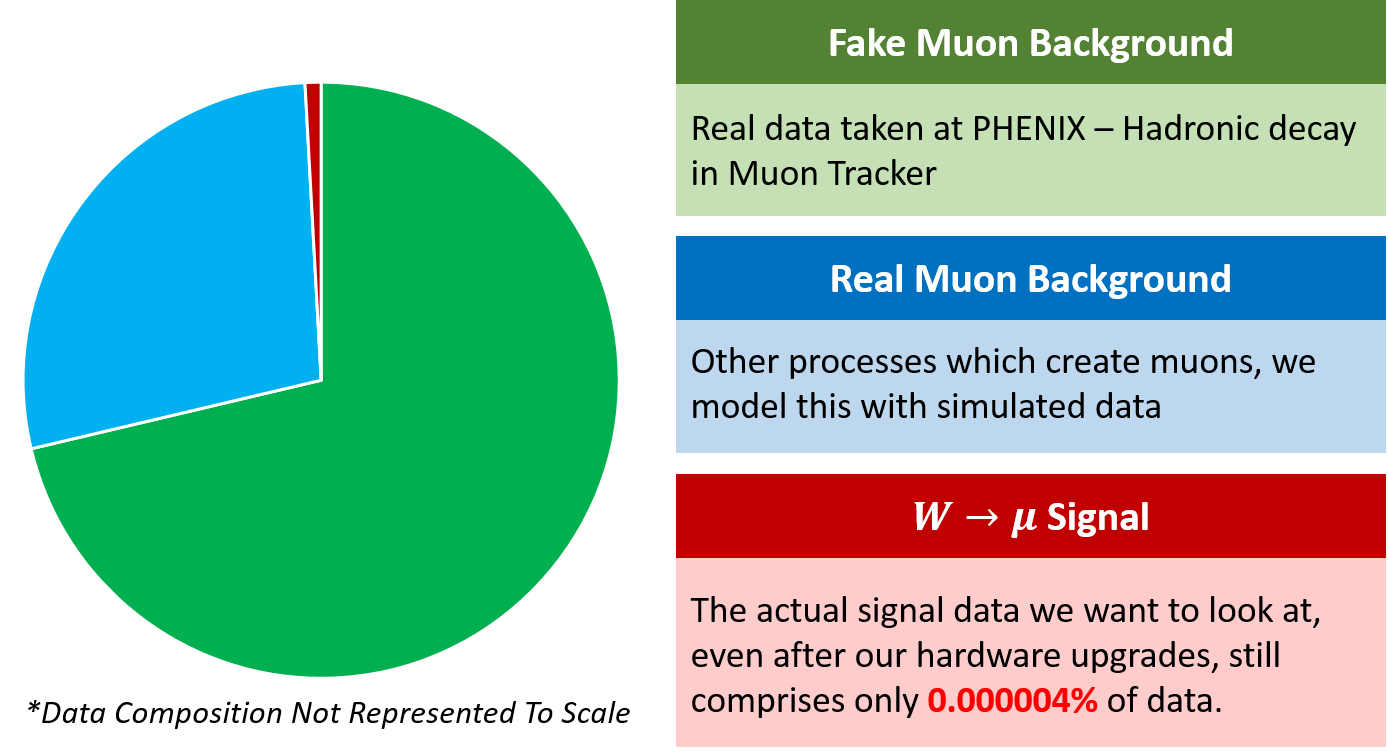
\includegraphics[width=0.8\linewidth]{./figures/data_composition.png}
  \caption{
    A cartoon of the dataset composition. The data, even after the Forward
    Upgrade, is mostly composed of hadronic background, which has tricked our
    Muon Tracker.
  }
  \label{fig:data_composition}
\end{figure}

In subsequent sections, I will discuss what we do with the variables which we
have chosen to use to identify W-genic events. Because our data set is so
dominated by background sources, we must rely heavily on simulations to estimate
what our signal events might look like. As of the time of this writing, the
analysis has not yet incorporated the simulation of hadronic background, which
is quite difficult, as there are a lot of effects at play - particles which
interact with the material of PHENIX itself to produce secondary and tertiary
vertices, for example. However, if we can simulate accurately the signal process
(the W-Boson cross section and its scaling with energy is known to excruciating
precision), and the muon background processes (known to similarly high
precision), we can approach the problem from a standpoint of using our data set
as a relatively good model for what 'hadronic background' looks like, and use
simulations to fit the portions of the data which cannot come from this hadronic
background. 

\clearpage
\section{The Basic Cut}

The basic cut aims to remove all obviously bad events from our event mix. The
cut approaches this from two premises. The first, is that if track
reconstruction variables simply cannot have resulted from a W-genic event, then
we remove the track. Secondly, if the track corresponds to a reconstructed
energy which is larger than what is physically allowable for a W-genic track, we
remove it.

The "Basic Cut" is defined:
\begin{table}[ht]
  \centering
  \begin{tabular}{l c c}
    \toprule
    \textbf{Variable} & \textbf{Lower Bound} & \textbf{Upper Bound} \\
    \midrule
    MuID lastGap & * & Gap 4 \\ 
    $\chi^2$ & 0 & 20 \\
    $DG0$ & 0 & 20 \\
    $DDG0$ & 0 & 9 \\
    $\mu$ candidate & * & 1 \\
    \bottomrule
  \end{tabular}
  \caption{ The Basic Cuts used in the Run 13 analysis. lastGap refers to the
    last gap in the MUID which saw a $\mu$ candidate event. The fourth gap is
    the furthest penetration possible, therefore suggesting a high energy muon.
    Other parameters are described in Tables \ref{tab:evt_variables}, 
    \ref{tab:mutr_variables}, \ref{tab:fvtx_variables}, and
    \ref{tab:rpc_variables}
  }
  \label{tab:basic_cut}
\end{table}

With this cut, we have removed quite a large fraction of background events from
our dataset without worry of removing any events in that fall within the
kinematic range of W-Boson production.

\clearpage
\section{Simulations}

I did not do any work to produce the simulations used in this analysis, all of
that credit goes to Dr. Ralf Seidl. I will generally describe how the
simulations were produced, and paraphrase from the analysis note which we
co-wrote with contributions also from Dr. Giordano, Abraham Meles and Daniel
Jumper:~\cite{Seidl2014a}.

PHENIX has a rather well developed simulation framework, which uses the in-house
built "PHENIX Integrated Simulation Application" (PISA)~\cite{Macguire1997}
custom simulation framework. The simulation framework models in great detail the
entire 12mx18mx18m volume of the PHENIX apparatus, as well as all the various
material properties of the apparatus. The software package originated from the
GEANT geometry and tracking packages. PISA encompasses more than this, though,
it additionally encapsulates event-generators, a standalone geometry
verification package, and the PHENIX offline analysis shell, to generate data
that is completely compatible with PHENIX's data packaging framework. PISA has
since been integrated into a simulation work-flow with the popular PYTHIA event
generation system.

The simulations were created by selecting the biggest sources of muon
background known to be produced at PHENIX as well as the W-Boson event and
producing many events to generate good statistics. The primary purpose of
simulating the muon background and W-Signal is to ultimately generate
probability distribution functions for the variables which have the largest
analyzing power - i.e. ability to differentiate between signal and background.
The simulation and data both are ultimately described by the same variables.

The data are added together, when combined to generate a 'muon background pdf'
or 'W-Signal pdf' according to the cross-section of the process and the number
of generated events, so as to not add these ingredients into the cocktail in the
wrong amounts. This process is described in the next section, but the
simulations used in this analysis are summarized here, in
Table~\ref{tab:simulation_cross_sections}. When adding the simulations together,
one must be careful to scale the final-yields by a correction factor (called
k-factor) such that events which produce boosted dimuons are properly accounted
for.

PHENIX uses some somewhat exclusive jargon when describing the various quark
bound states which contribute to the muon background, and signal events.  Open
charm or charmonium refer to the bound state of the $c\bar{c}$ quarks.  Onium
generally refers to any process where a particle is in a bound-state with its
own antiparticle (without of course double-counting open charm/charmonoim).
Direct photon, or alternatively $d\gamma$ (sometimes also written as DY) refers
to photons that are produced as an immediate result of a inelastic scattering
process, not from secondary decays. Open bottom refers to the bound state of
$b\bar{b}$ quarks. Z/$d\gamma$ refers to the production and decay of the mixing
between the Z-boson and virtual photons. ONLY Z refers to Z production and
decay.  W is naturally the signal event. W tau refers to the production of tau
leptons, which can decay weakly, producing electrons or muons. W had refers to
the production of W bosons from hadronic processes, rather than as the primary
event vertex.  All of these processes are summarized in
Table~\ref{tab:simulation_cross_sections}.  
\begin{table}[ht]
  \centering
  \begin{tabular}{ccccc}
    \toprule
    \multicolumn{5}{c}{\textbf{Reference Run 393888}}\\ 
     & & & & \\
    \textbf{Process} & 
    \textbf{k factor} & 
    \textbf{$\sigma$ } & 
    \textbf{\# Events} & 
    \textbf{ $\mathcal{L}$ } \\
    & & (\textit{mb}) &  & ($fb^{-1}$) \\
    \midrule
    $c\bar{c}$ & 2.44  & 5.71e-01 & 5.85e+11 & 1.02 \\
    onium      & 0.415 & 1.35e-01 &  1.5e+11 & 1.11 \\
    $d\gamma$  & 0.0   & 5.32e-02 & 5.84e+10 & 1.10 \\
    $b\bar{b}$ & 1.83  & 7.30e-03 & 7.36e+09 & 1.01 \\
    ONLY Z     & 1.25  & 3.37e-07 & 1.73e+08 & 577.0\\
    W          & 1.5   & 1.66e-06 & 3.38e+08 & 198.9\\
    W tau      & 0.0   & 1.66e-06 & 3.43e+08 & 201.8\\
    W had      & 0.0   & 1.66e-06 & 3.42e+08 & 201.2\\
    Z          & 1.25  & 1.02e-06 & 2.93e+08 & 61.2 \\
    \bottomrule
  \end{tabular}
  \caption{
    Simulated sub processes in Run 13 including their generated event numbers
    as well as the corresponding luminosity and cross sections. Dr. Sanghwa Park
    has done an extensive analysis of the simulated data to determine an
    appropriate k-factor. Process which contribute very little to the muon
    background include W had, W tau, and $d\gamma$; they are scaled to zero.
  }
  \label{tab:simulation_cross_sections}
\end{table}                  


The simulations must additionally be weighted for trigger efficiency. To
accomplish this, we weight events for each arm and charge with the associated
trigger efficiency when constructing probability density functions representing
the muon background. The trigger efficiencies generally manifest as $\eta$
dependent functions - thus we bin the data into 20 separate $\eta$ bins and
calculate the efficiency associated with each bin. The bin ranges, and
efficiency corrections are summarized in
Table~\ref{tab:rapidity_corrections_north} for the North arm, and
Table~\ref{tab:rapidity_corrections_south} for the South arm.
\begin{table}
  \centering
  \begin{tabular}{cccc}
    \toprule
    \multicolumn{4}{c}{\textbf{South Arm}} \\
    \textbf{$\eta_{min}$} & 
    \textbf{$\eta_{min}$} & 
    \textbf{$\mu^{-}\pm stat \pm sys$} & 
    \textbf{$\mu^{+}\pm stat \pm sys$} \\
    \midrule
    1.10 & 1.17 & $0.27912 \pm 0.00297 \pm 0.10243$ & $0.30607 \pm 0.00423 \pm 0.01108$ \\
    1.17 & 1.25 & $0.40422 \pm 0.01642 \pm 0.04811$ & $0.43125 \pm 0.01717 \pm 0.26702$ \\
    1.25 & 1.32 & $0.27958 \pm 0.00056 \pm 0.05539$ & $0.36619 \pm 0.00925 \pm 0.07316$ \\
    1.32 & 1.40 & $0.26563 \pm 0.00542 \pm 0.02485$ & $0.25312 \pm 0.00349 \pm 0.04927$ \\
    1.40 & 1.48 & $0.39802 \pm 0.00497 \pm 0.07770$ & $0.34295 \pm 0.00306 \pm 0.03127$ \\
    1.48 & 1.55 & $0.43156 \pm 0.00633 \pm 0.17060$ & $0.37567 \pm 0.00248 \pm 0.03644$ \\
    1.55 & 1.62 & $0.34831 \pm 0.00309 \pm 0.03720$ & $0.40246 \pm 0.00546 \pm 0.04605$ \\
    1.62 & 1.70 & $0.33043 \pm 0.00280 \pm 0.09227$ & $0.40219 \pm 0.00472 \pm 0.05637$ \\
    1.70 & 1.77 & $0.33152 \pm 0.00318 \pm 0.11668$ & $0.30805 \pm 0.00360 \pm 0.03644$ \\
    1.77 & 1.85 & $0.34710 \pm 0.00633 \pm 0.00918$ & $0.38565 \pm 0.00439 \pm 0.04295$ \\
    1.85 & 1.92 & $0.32448 \pm 0.00404 \pm 0.14670$ & $0.30118 \pm 0.00418 \pm 0.10071$ \\
    1.92 & 2.00 & $0.31461 \pm 0.00714 \pm 0.01799$ & $0.31263 \pm 0.00545 \pm 0.01643$ \\
    2.00 & 2.07 & $0.64632 \pm 0.01161 \pm 0.23329$ & $0.63252 \pm 0.01040 \pm 0.10507$ \\
    2.07 & 2.15 & $0.60582 \pm 0.00565 \pm 0.05569$ & $0.67335 \pm 0.01245 \pm 0.05630$ \\
    2.15 & 2.22 & $0.45058 \pm 0.00697 \pm 0.45101$ & $0.69619 \pm 0.01247 \pm 0.65623$ \\
    2.22 & 2.30 & $0.45185 \pm 0.01358 \pm 0.36032$ & $0.51436 \pm 0.01288 \pm 0.43781$ \\
    2.30 & 2.38 & $0.43890 \pm 0.07336 \pm 0.34632$ & $0.61623 \pm 0.06221 \pm 0.62209$ \\
    2.38 & 2.45 & $0.00000 \pm 0.25000 \pm 0.00000$ & $0.00000 \pm 0.25000 \pm 0.00000$ \\
    2.45 & 2.52 & $0.00000 \pm 0.25000 \pm 0.00000$ & $0.00000 \pm 0.25000 \pm 0.00000$ \\
    2.52 & 2.60 & $0.00000 \pm 0.25000 \pm 0.00000$ & $0.00000 \pm 0.25000 \pm 0.00000$ \\
    \bottomrule
  \end{tabular}
  \caption{
    $\eta$ dependent trigger efficiencies are calculated for the South arm in 20
    $\eta$ bins. Each correction has both systematic and statistical error
    accounted for.
  }
  \label{tab:rapidity_corrections_south}
\end{table}

\begin{table}
  \centering
  \begin{tabular}{cccc}
    \toprule
    \multicolumn{4}{c}{\textbf{North Arm}} \\
    \textbf{$\eta_{min}$} & 
    \textbf{$\eta_{min}$} & 
    \textbf{$\mu^{-}\pm stat \pm sys$} & 
    \textbf{$\mu^{+}\pm stat \pm sys$} \\
    \midrule
    1.10 & 1.17 & $0.56285 \pm 0.03834 \pm 0.32882$ & $0.52850 \pm 0.01938 \pm 0.36163$ \\
    1.17 & 1.25 & $0.67803 \pm 0.02249 \pm 0.13431$ & $0.49546 \pm 0.00261 \pm 0.16304$ \\
    1.25 & 1.32 & $0.69537 \pm 0.01551 \pm 0.03465$ & $0.63287 \pm 0.01285 \pm 0.08350$ \\
    1.32 & 1.40 & $0.39864 \pm 0.00724 \pm 0.02330$ & $0.38435 \pm 0.00762 \pm 0.11954$ \\
    1.40 & 1.48 & $0.52102 \pm 0.00750 \pm 0.05014$ & $0.49573 \pm 0.00698 \pm 0.03733$ \\
    1.48 & 1.55 & $0.48068 \pm 0.00498 \pm 0.11579$ & $0.48874 \pm 0.00357 \pm 0.08063$ \\
    1.55 & 1.62 & $0.54113 \pm 0.00860 \pm 0.04895$ & $0.50041 \pm 0.00659 \pm 0.05165$ \\
    1.62 & 1.70 & $0.45140 \pm 0.00822 \pm 0.05718$ & $0.46948 \pm 0.00755 \pm 0.09718$ \\
    1.70 & 1.77 & $0.43203 \pm 0.00547 \pm 0.04976$ & $0.40722 \pm 0.00546 \pm 0.07957$ \\
    1.77 & 1.85 & $0.42141 \pm 0.00815 \pm 0.04366$ & $0.44450 \pm 0.00628 \pm 0.04575$ \\
    1.85 & 1.92 & $0.37946 \pm 0.00620 \pm 0.01766$ & $0.37183 \pm 0.00700 \pm 0.01848$ \\
    1.92 & 2.00 & $0.37499 \pm 0.00782 \pm 0.05026$ & $0.40156 \pm 0.00678 \pm 0.02291$ \\
    2.00 & 2.07 & $0.51268 \pm 0.00547 \pm 0.10416$ & $0.60041 \pm 0.00973 \pm 0.21212$ \\
    2.07 & 2.15 & $0.56990 \pm 0.00614 \pm 0.14507$ & $0.58276 \pm 0.01392 \pm 0.25179$ \\
    2.15 & 2.22 & $0.60527 \pm 0.01524 \pm 0.10354$ & $0.60766 \pm 0.00425 \pm 0.23618$ \\
    2.22 & 2.30 & $0.70200 \pm 0.01678 \pm 0.25233$ & $0.45067 \pm 0.01008 \pm 0.24192$ \\
    2.30 & 2.38 & $0.48294 \pm 0.00294 \pm 0.12663$ & $0.54157 \pm 0.02109 \pm 0.06230$ \\
    2.38 & 2.45 & $0.47814 \pm 0.02338 \pm 0.42026$ & $0.42606 \pm 0.03092 \pm 0.25031$ \\
    2.45 & 2.52 & $0.61788 \pm 0.14438 \pm 0.61788$ & $0.29673 \pm 0.06686 \pm 0.04941$ \\
    2.52 & 2.60 & $0.00000 \pm 0.25000 \pm 0.00000$ & $0.15630 \pm 0.15630 \pm 0.18223$ \\
    \bottomrule
  \end{tabular}
  \caption{
    $\eta$ dependent trigger efficiencies are calculated for the North arm in 20
    $\eta$ bins. Each correction has both systematic and statistical error
    accounted for.
  }
  \label{tab:rapidity_corrections_north}
\end{table}

We can visualize the composition of the simulated data set by stacking the
relative distributions of these variables. By looking the cross-sections of
these variables as a function of $p_T$, for each arm and charge combination, we
can get a feeling for how the data set composition varies with $p_T$
(Figure~\ref{fig:stacked_xsec_sim}).

\begin{figure}[ht]

  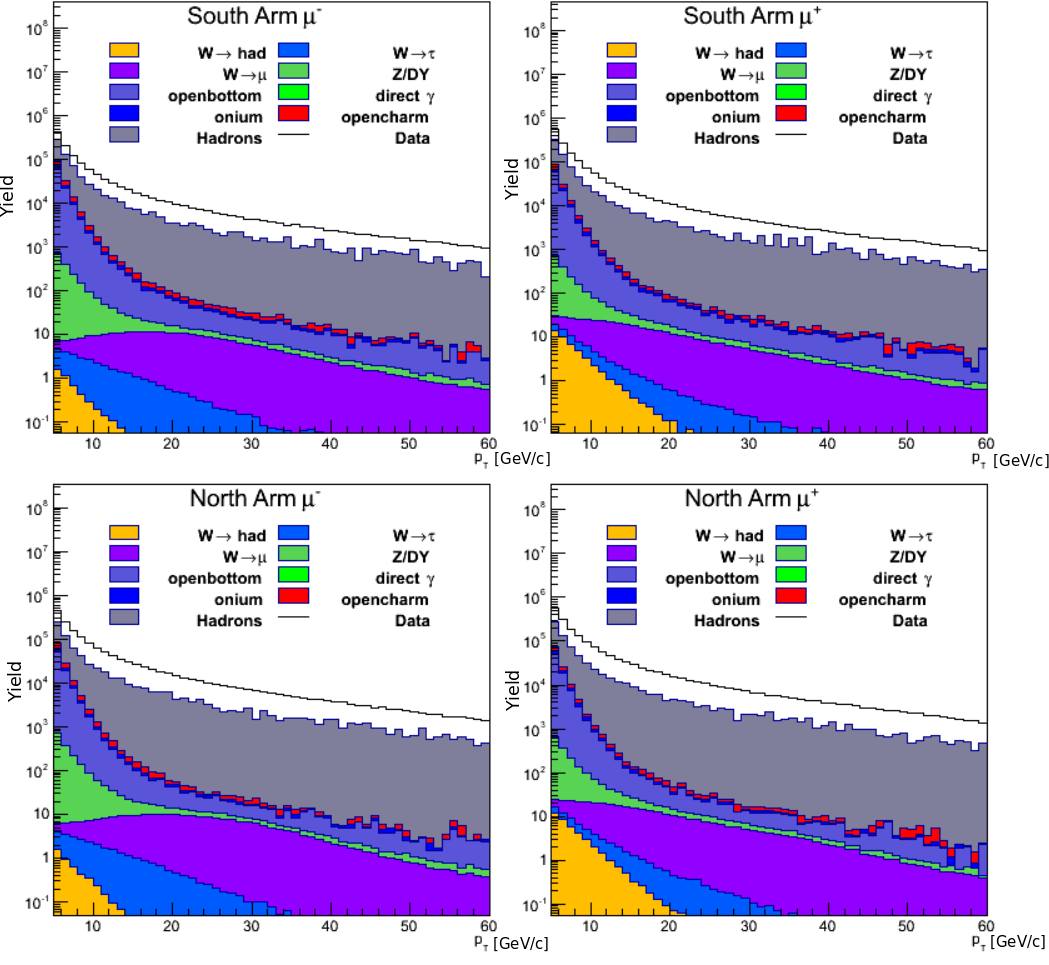
\includegraphics[width=\linewidth]{./figures/stacked_xsec.png}
  \caption{
    Here, we see the stacked cross-sections of all simulated processes as a
    function of $p_T$. All data shown has been created from the PISA+PYTHIA
    framework. Top Left: South $\mu-$, Top Right: South $\mu+$, Bottom Left:
    North $\mu+$, Bottom Right: North $\mu-$. Figure reproduced from my analysis
    note. Dr. Ralf Seidl produced the original ~\cite{Seidl2014a}
  }
  \label{fig:stacked_xsec_sim}
\end{figure}

\clearpage


\section{$W_{ness}$: Likelihood Event Tagging}
\label{sec:likelihood}

Recalling that we have already split the dataset into three main contributions:
hadronic background, real muon background, and W-Signal, we are now tasked with
formulating a means to separate signal from background, using the variables
which can indicate the straight-ness of a muon track.

Previous analyses have attempted to separate the muon spectrum into $p_T$ bins,
to estimate the composition, however, because the $W\rightarrow\mu$ signal is so
small in the forward kinematic regime, these methods are not sufficient, as
there is no 'visible' cutoff in the spectrum.

However, we may use other methods to split up our spectrum, with the ultimate
goal of calculating $A_L$, and correcting for background dilution using the
signal to background ratio. We must use another method to effectively describe
the difference between an event which comes from a signal, vs background event.

We expect that tracks which are straight are more likely to come from a W-Boson
decay, because this indicates high momentum. One way of thinking of our data set
can in terms of a classification problem. In a classification problem, one can
use Bayes Theorem when one has a labeled testing data set to build predictive
models which can classify data into two or more classes, provided that care is
taken to not over-train the classifier, or attempt to classify data which has
been used in the subset of data to train the classifier.

In our case, we have simulations which serve as the training data, guaranteeing
that there will be no overlap between the physical data produced, and the data
used to train the classifier. Thus, we implement a Naive Bayes Classifier (also
known as Likelihood Selection) to label our data with two classes. Rather than
labeling data with a binary classification, however, we opt to label the data
with its likelihood, a posterior probability which tells us if a value is more
or less likely to come from a W-Boson.

\subsection{Naive Bayes Classification}
There are many techniques available for classifying a collection of variables
(a feature set) into categories. Naive Bayes classification is an excellent
candidate for classification, in cases where we have two classifications with
distributions of feature sets which are uncorrelated. Naive Bayes even works when
feature sets are slightly correlated. It is a robust, fast, scalable machine
learning technique. Traditionally used for classification of text documents,
Naive Bayes is also able to handle numeric features whose distributions are
known \cite{Collins2013}.

In our analysis, we begin with a Naive Bayes classifier which is trained to
classify signal muons or background muons. We combine both Real Muon
Background muons and Fake Muons (Hadronic Background Muons) in the label of
"Background Muons" at this stage, though, later, we will separate out the muons
further.

In order to obtain the best performance from our classifier, without
over-training, we need to ensure that the variables (or feature set) used to
determine a class are maximally uncorrelated. The variables which match this
criteria are: DG0, DDG0, $\chi^2$, $fvtx$ variables, Rpc1DCA, Rpc3DCA, DCA$_r$,
and DCA$_z$. The Linear Correlations between these variables are shown for both
the data, and the simulated W-Signal in
Figure~\ref{fig:kinematic_var_correlations}.

\begin{figure}[H]
	\centering
	\begin{subfigure}[t]{0.5\textwidth}
		\centering
		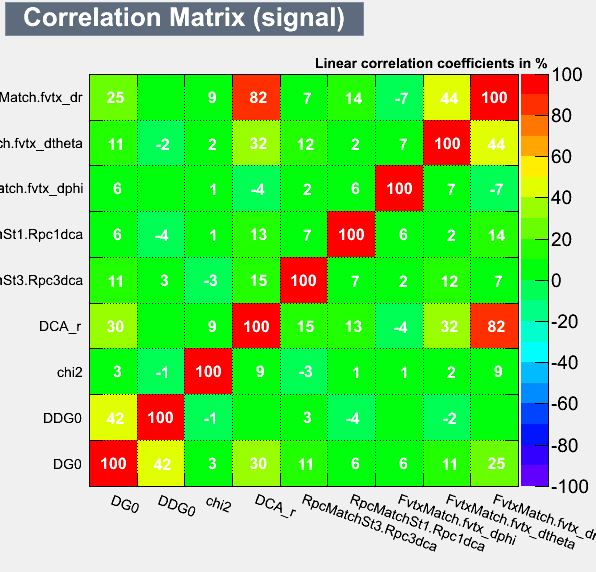
\includegraphics[width=0.95\linewidth]{./figures/CorrelationMatrix_Signal.png}
		\caption{Correlations between kinematic variables, produced from simulated
			data.}
		\label{fig:corr_mat_sig}
	\end{subfigure}%
  \begin{subfigure}[t]{0.5\textwidth}
		\centering
		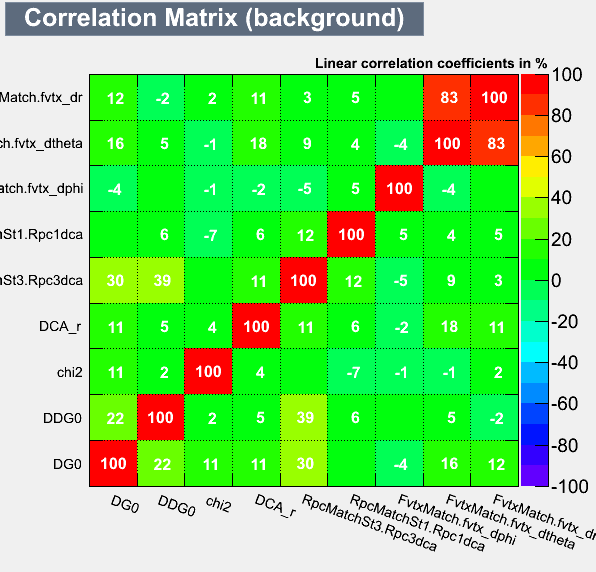
\includegraphics[width=0.95\linewidth]{./figures/CorrelationMatrix_Background.png}
		\caption{Correlations between kinematic variables, produced from the data,
			which is composed mostly of hadronic background}
		\label{fig:corr_mat_bkg}
	\end{subfigure}
	\caption{ Low correlations between the signal variable distributions (from
		simulation), and the background variable distributions make this data set a
		good candidate for classification using Naive Bayes}
	\label{fig:kinematic_var_correlations}
\end{figure}

As one can see from Figure~\ref{fig:kinematic_var_correlations}, DG0 and DDG0
are slightly correlated, as are $chi^2$ and DCA$_r$. A Naive Bayes classifier
may be constructed from the core of the familiar Bayes Theorem from probability
and statistics. In our case, we understand Naive Bayes as a conditional
probability. Concretely, we consider a vector of features (i.e.  our
discriminating kinematic variables):

\begin{equation}
	\label{eq:feature_vector}
\mathbf{x} = (x_1, \dots, x_n)
\end{equation}

and assume independence between each feature $x_n$. We then define the
probability of a given classification, $C_k$ given a set of features $x_n$:

\begin{equation}
	\label{eq:cond_probabilty}
  \mathcal{P}(C_k \vert x_1, \dots, x_n)
\end{equation}

This conditional probability is defined in terms of Bayes Theorem:

\begin{equation}
	\label{eq:bayes_theorm}
  \mathcal{P}(C_k \vert \mathbf{x}) = \frac{\mathcal{P}(C_k) \
  \mathcal{P}(\mathbf{x} \vert C_k)}{\mathcal{P}(\mathbf{x})}
\end{equation}

The terms here are defined as:
\begin{itemize}
  \item $\mathcal{P}(C_k)\rightarrow$ prior probability
	\item $\mathcal{P}(\mathbf{x} \vert C_k)\rightarrow$ likelihood
	\item $\mathcal{P}(\mathbf{x})\rightarrow$ evidence
\end{itemize}

The probabilities described here are realized through constructing probability
density functions from the data and simulations. The constraints of these
probability distribution functions is that they are well behaved in the sense
that they are finite and convergent in asymptotic limits, such that they can be
meaningfully normalized.

In our case, we construct a likelihood ratio, using the posterior probability
for each classification, which is defined as $W_{ness}$:
\begin{align*}
  \lambda_{sig} &= \prod_{k}\mathcal{P}(\mu_{sig}\vert C_k)\\
  \lambda_{bak} &= \prod_{k}\mathcal{P}(\mu_{bak}\vert C_k)
\end{align*}

Where $\lambda_{sig}$ and $\lambda_{bak}$ represent the total likelihoods that a
given track is either signal, or background, constructed from the product of
likelihoods calculated from each probability density function. The $\lambda$'s
are combined to calculate the $W_{ness}$:

\begin{equation}
  W_{ness} = { 
    {\lambda_{sig}}
    \over 
    {\lambda_{sig}+\lambda_{bak}} 
  }
\end{equation}


Thus, we must construct probability density functions representing the
likelihood of an event being W-genic or from the combined hadronic+muon
background. Our data set after th basic cut has approximately 1 million events.
Based on the cross-section of the $W\rightarrow \mu$ decay, we expect the final
population of W-Bosons in the data set to be on the order of 1 thousand.
Therefore, we can confidently use the data set as is, in order to generate PDFs
representing the hadronic+muon background, as any effect from the signal would
be only one part in a thousand. Thus, we loop over the data set, and the
W-Simulation set, and filter the data into probability distribution functions.
Because some events do not have archived data from all subsystems, we construct
a variety of PDFs, selecting the appropriate PDF cocktail based on whether or
not the requisite variables were archived for that given track,
Figure~\ref{fig:pdf_selection_tree}.

\begin{figure}[ht]
  \centering
  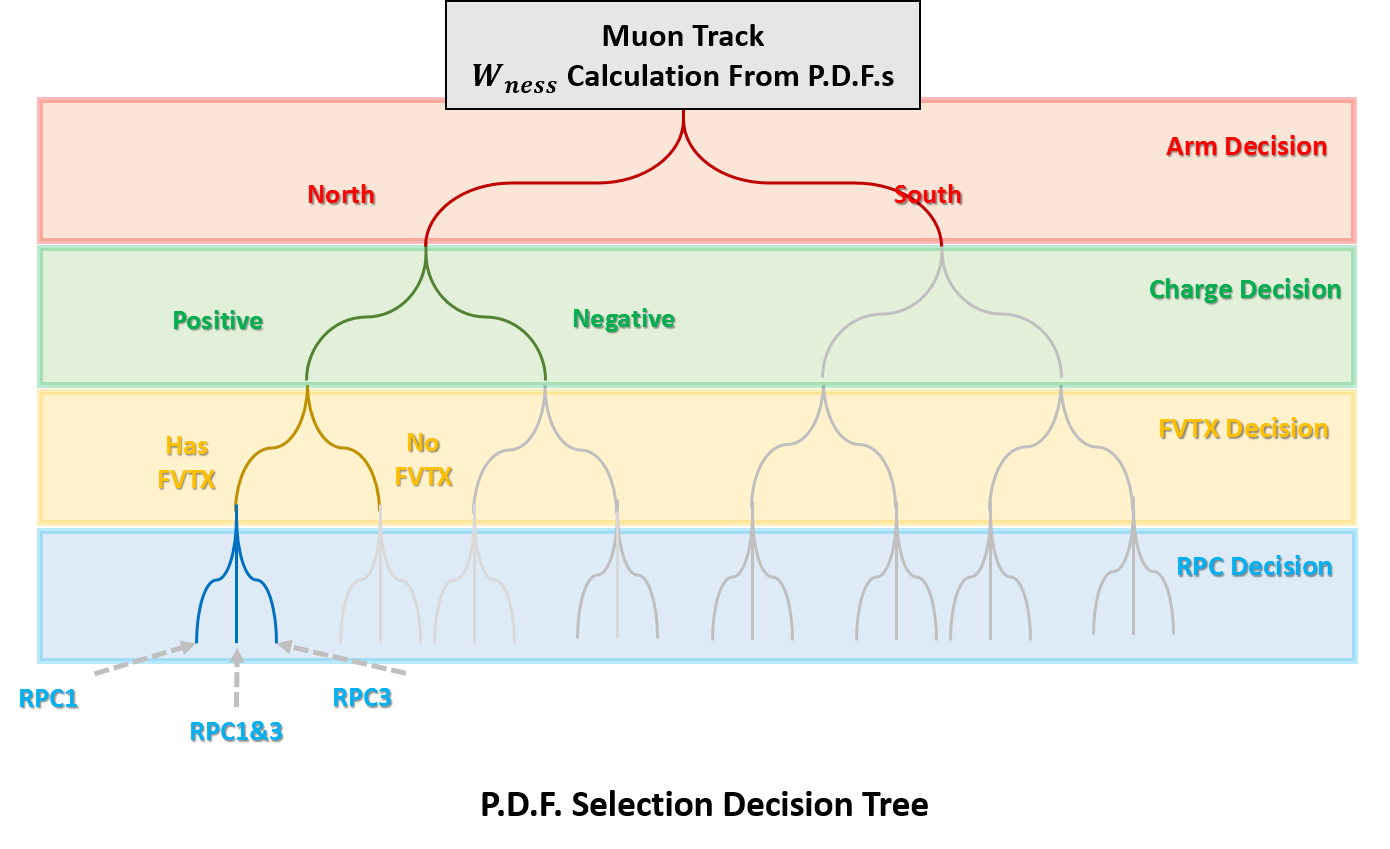
\includegraphics[width=\linewidth,trim=4 4 4 4,clip]{./figures/pdf_selection_tree.png}
  \caption{
    A cartoon of the decision tree to determine the PDF cocktail to use for
    quantifying the $W_{ness}$ of a given track. The track's properties are used
    to traverse the tree, and select the cocktail contents.
  }
  \label{fig:pdf_selection_tree}
\end{figure}

In figures~\ref{fig:pdf_rpc3dca}-\ref{fig:pdf_DG0}, we can see the various
distributions which are used to create probability distribution functions. In
the figures, we represent the product of all probability functions which are
used to tag an event as $\lambda$ such that 
$\lambda = \Pi_{k} \mathcal{P}(\mu \vert C_k)$.

\begin{figure}
  \centering
  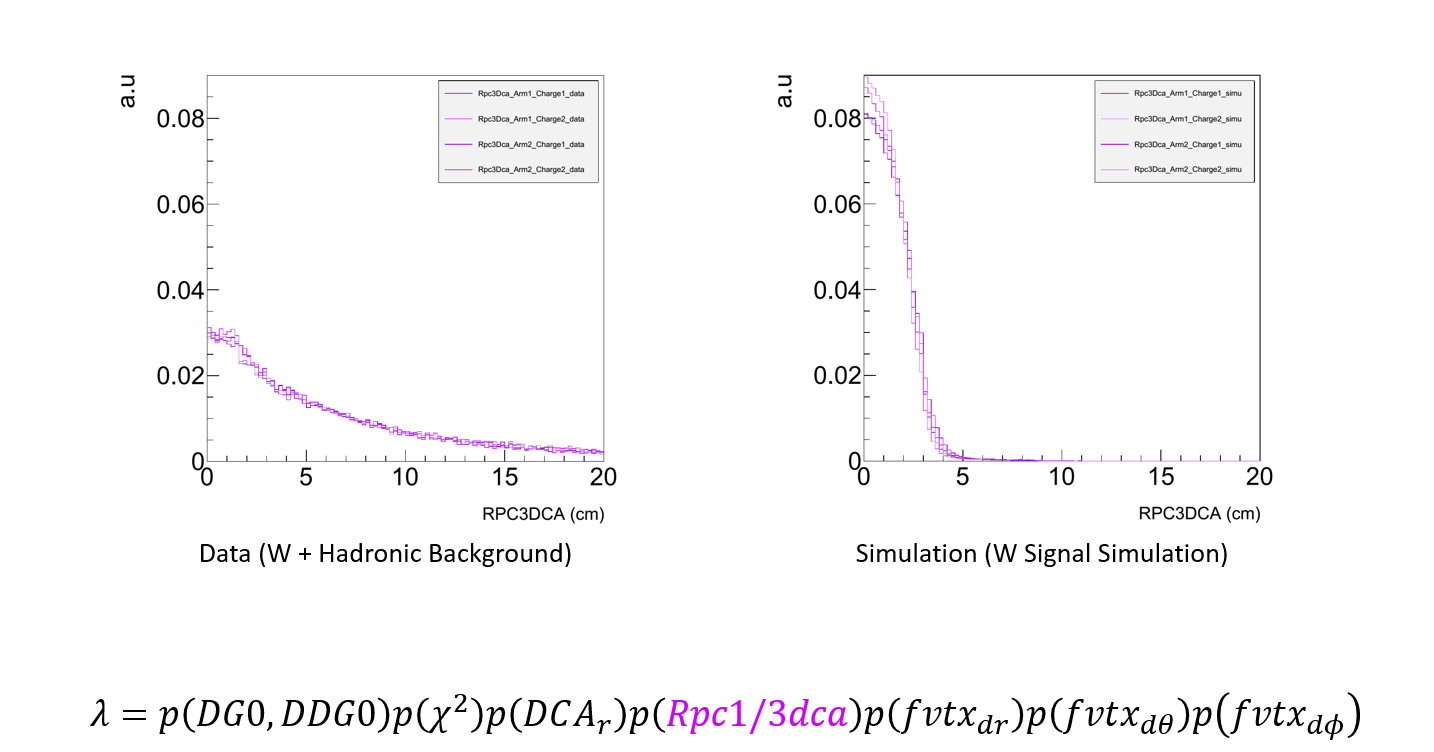
\includegraphics[width=\linewidth,trim=4 4 4 4,clip]{./figures/pdf_rpc3dca.png}
  \caption{
    Left: the distribution of Rpc3dca for each arm and charge, produced from the
    PHENIX data set, after the basic cut. Right: the same distributions from a
    simulation of the W-Signal.
  }
  \label{fig:pdf_rpc3dca}
\end{figure}

\begin{figure}
  \centering
  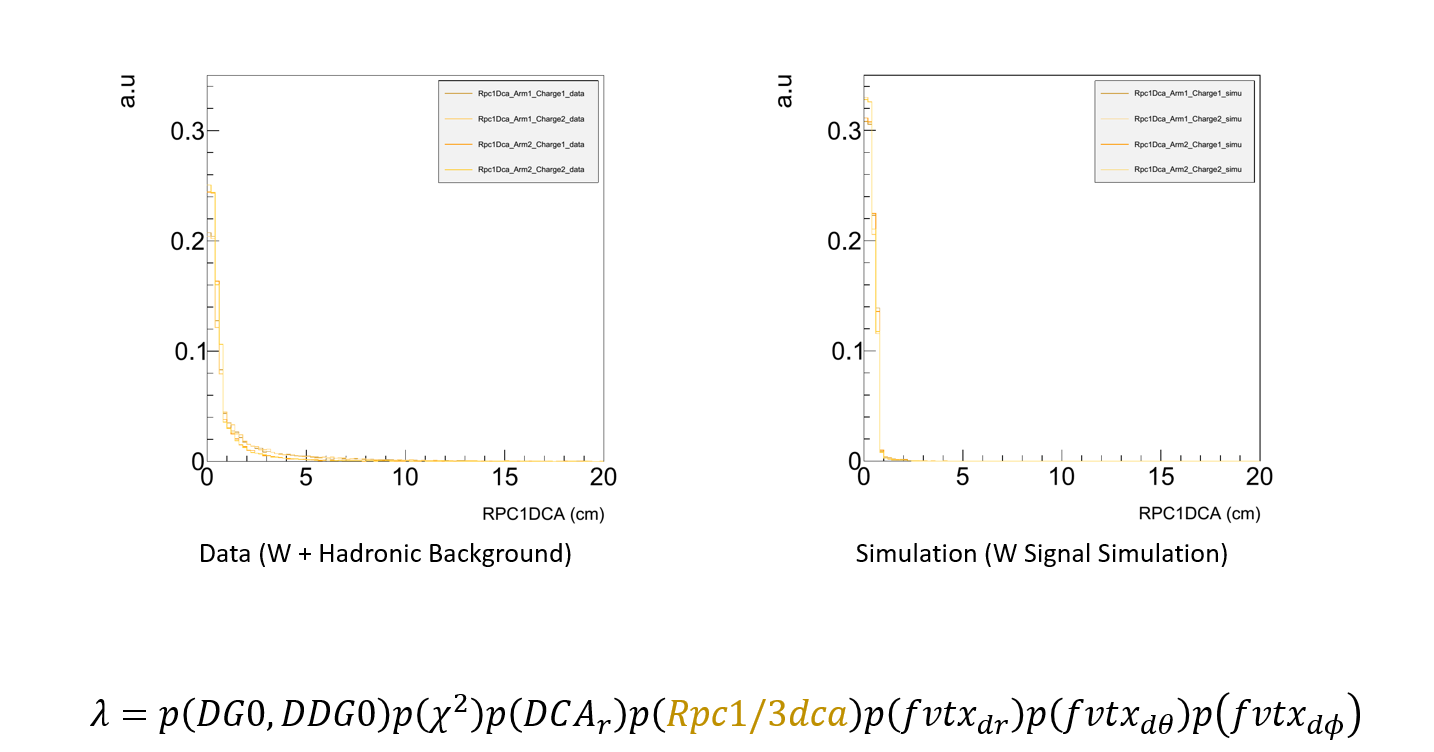
\includegraphics[width=\linewidth,trim=4 4 4 4,clip]{./figures/pdf_rpc1dca.png}
  \caption{
    Left: the distribution of Rpc1dca for each arm and charge, produced from the
    PHENIX data set, after the basic cut. Right: the same distributions from a
    simulation of the W-Signal.
  }
  \label{fig:pdf_rpc1dca}
\end{figure}

\begin{figure}
  \centering
  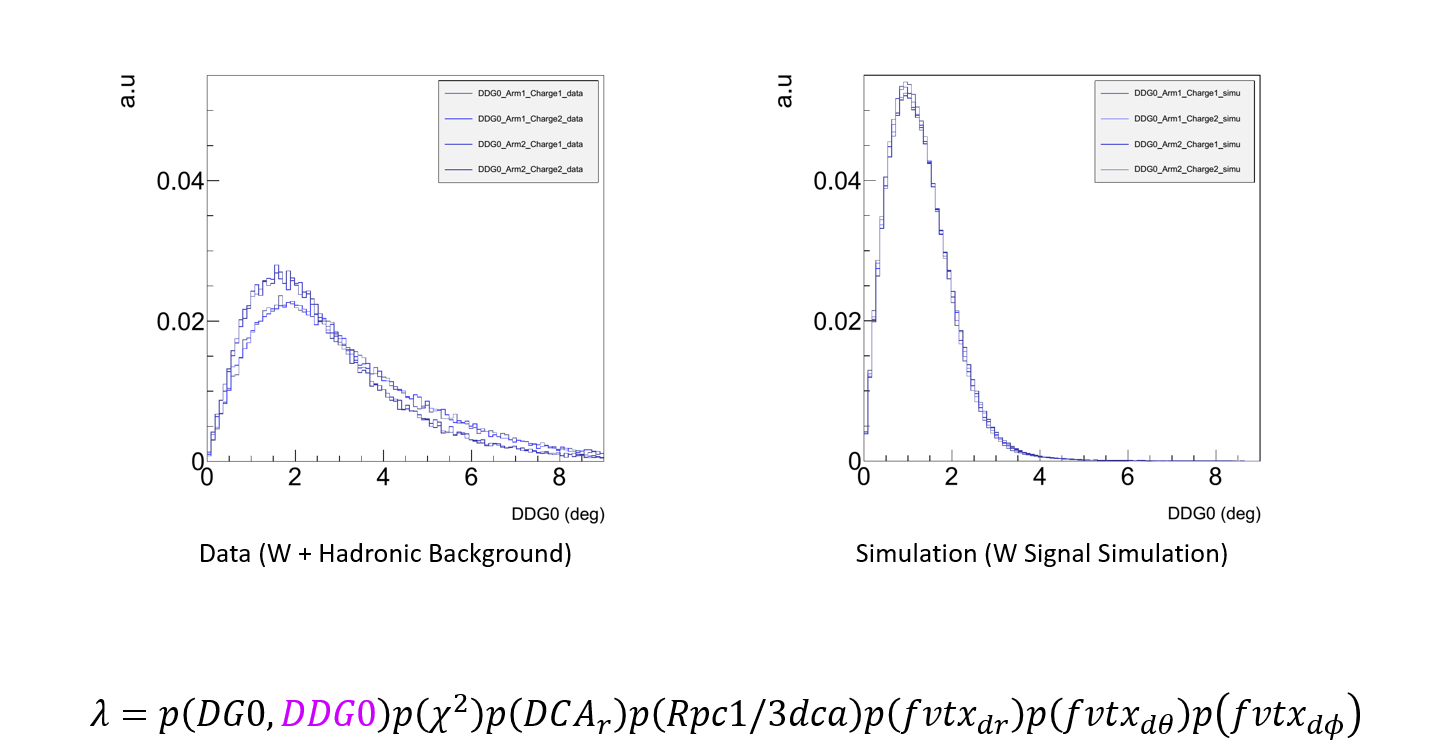
\includegraphics[width=\linewidth,trim=4 4 4 4,clip]{./figures/pdf_DDG0.png}
  \caption{
    Left: the distribution of DDG0 for each arm and charge, produced from the
    PHENIX data set, after the basic cut. Right: the same distributions from a
    simulation of the W-Signal.
  }
  \label{fig:pdf_DDG0}
\end{figure}

\begin{figure}
  \centering
  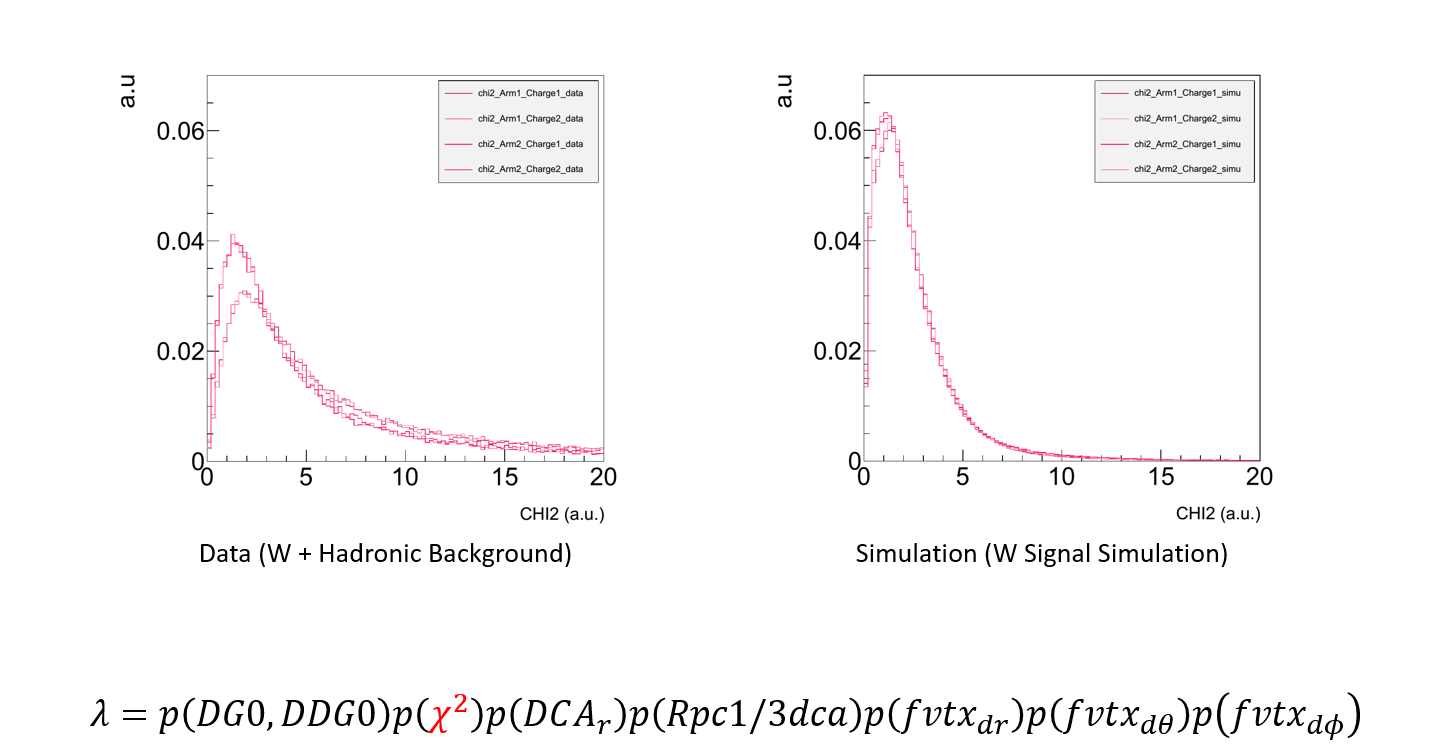
\includegraphics[width=\linewidth,trim=4 4 4 4,clip]{./figures/pdf_chi2.png}
  \caption{
    Left: the distribution of $\chi^2$ for each arm and charge, produced from the
    PHENIX data set, after the basic cut. Right: the same distributions from a
    simulation of the W-Signal.
  }
  \label{fig:pdf_chi2}
\end{figure}

\begin{figure}
  \centering
  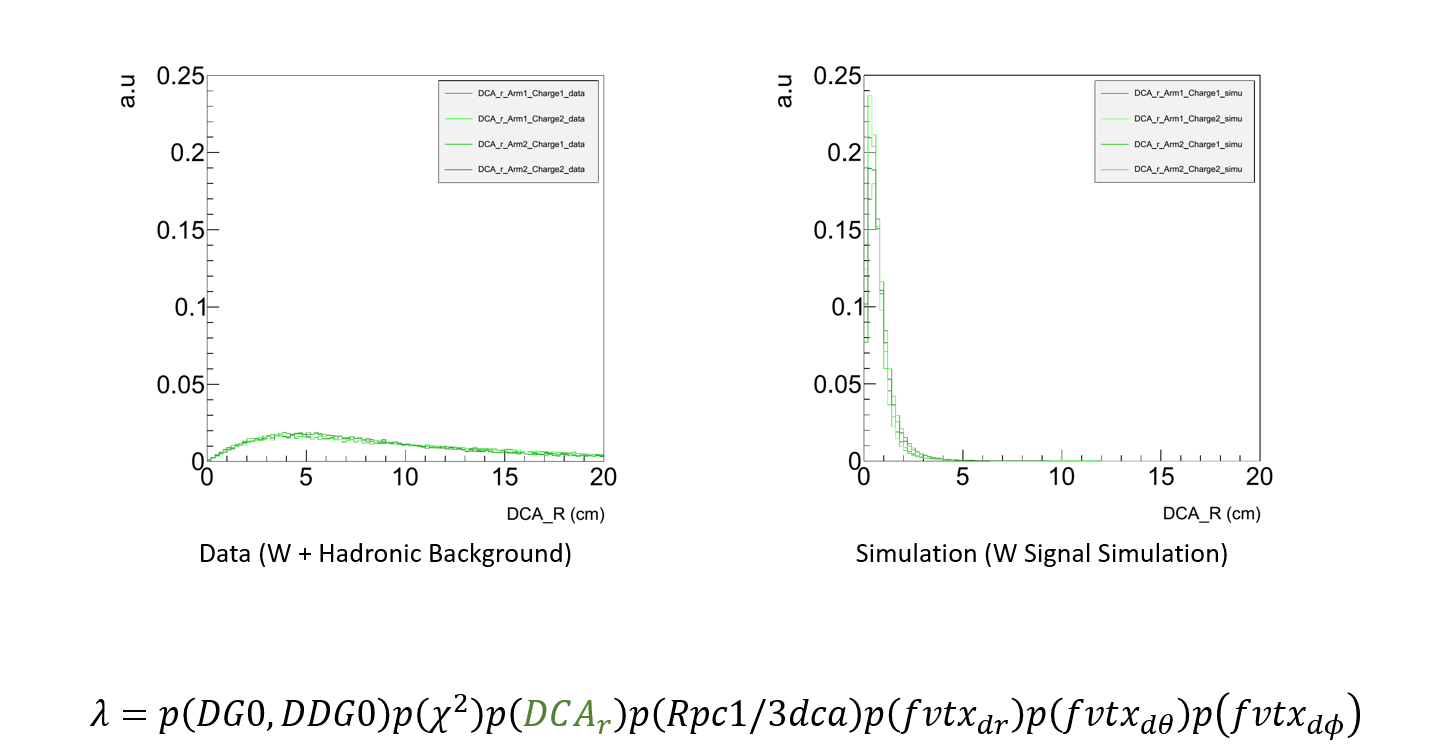
\includegraphics[width=\linewidth,trim=4 4 4 4,clip]{./figures/pdf_dcar.png}
  \caption{
    Left: the distribution of DCA$_r$ for each arm and charge, produced from the
    PHENIX data set, after the basic cut. Right: the same distributions from a
    simulation of the W-Signal.
  }
  \label{fig:pdf_dcar}
\end{figure}

\begin{figure}
  \centering
  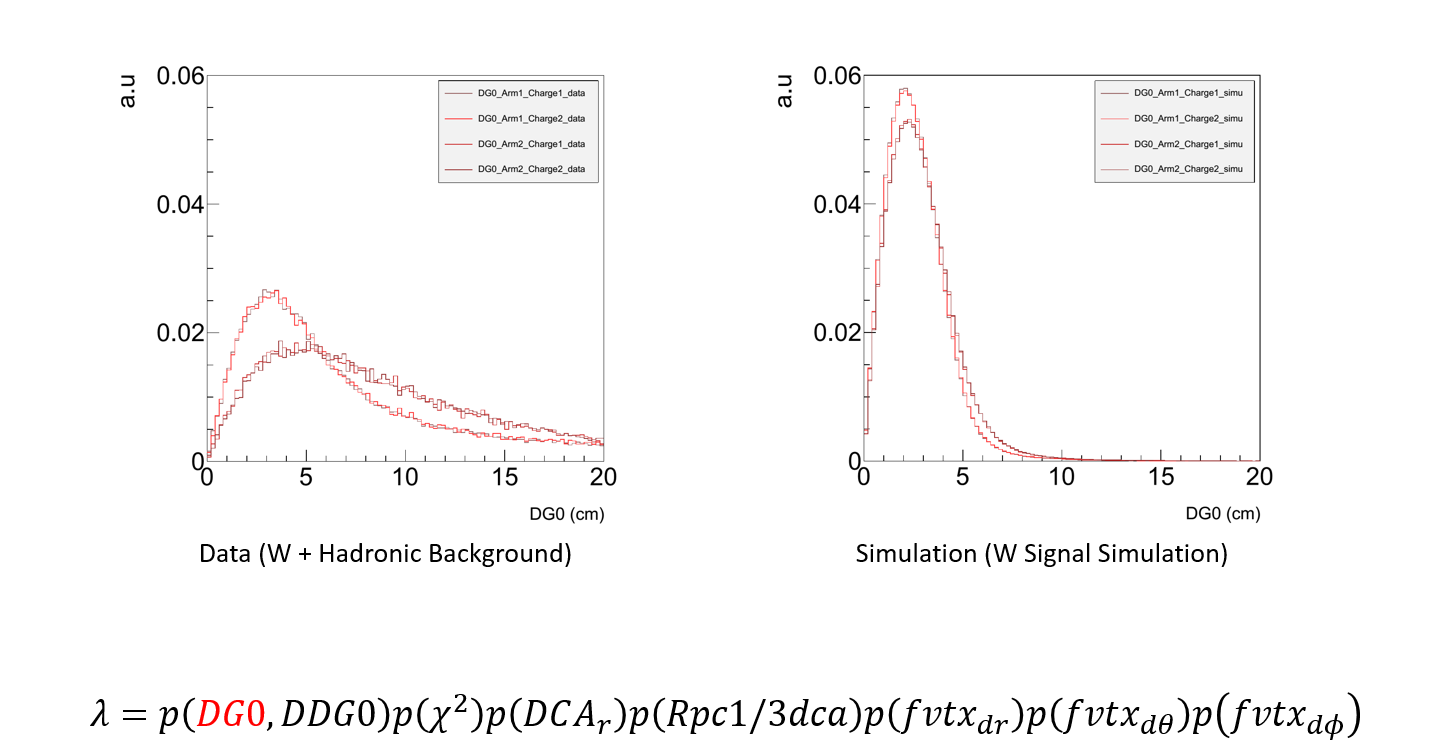
\includegraphics[width=\linewidth,trim=4 4 4 4,clip]{./figures/pdf_DG0.png}
  \caption{
    Left: the distribution of DG0 for each arm and charge, produced from the
    PHENIX data set, after the basic cut. Right: the same distributions from a
    simulation of the W-Signal.
  }
  \label{fig:pdf_DG0}
\end{figure}

Now that we have a complete set of probability density functions which predict
the likelihood that a given track is a W-genic muon or not, we can loop over the
real physics data set, and use our likelihood calculation strategy to label
every muon track with a $W_{ness}$. We may also tag our simulated data set with
$W_{ness}$. The distributions are shown in
Figure~\ref{fig:wness_distribution}.

\begin{figure}
  \centering
  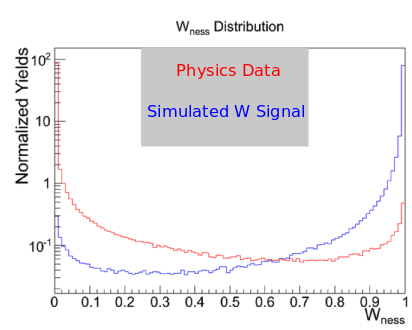
\includegraphics[width=0.7\linewidth]{./figures/wness_sig_bak.png}
  \caption{
    After $W_{ness}$ tagging, we can visualize the classification of signal from
    background by comparing the distribution of $W_{ness}$ in
    \textcolor{red}{physics data}, and the \textcolor{blue}{simulated data}
    data. Note that the vertical is plotted on a log scale. The two
    distributions have been normalized prior to plotting.
  }
  \label{fig:wness_distribution}
\end{figure}

As we can see from Figure~\ref{fig:wness_distribution}, most of the simulated
data falls in the high $W_{ness}$ range while most of the physics data falls in
the low $W_{ness}$ range. The goal of the likelihood analysis is to tag the data
with $W_{ness}$ such that we can apply a cut on the data based on the
parameter's value. We wish to apply the cut in a way that minimally removes any
signal, and we may calculate the efficiency of this cut, summarized in
Figure~\ref{fig:wness_cut_efficiency}.

\begin{figure}
  \centering
  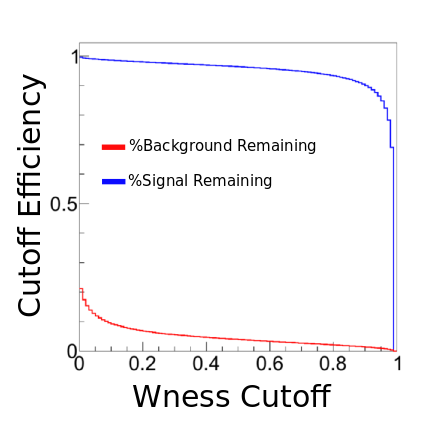
\includegraphics[width=0.7\linewidth]{./figures/wness_cut_efficiency.png}
  \caption{
    We look at the fraction of signal and background remaining in the total data
    set as we make successively higher cuts in $W_{ness}$. At the turning point
    of the blue distribution (the fraction of remaining signal) is where we
    choose to cut the data, corresponding to removing data with a $W_{ness}$
    value of less than 0.95.
  }
  \label{fig:wness_cut_efficiency}
\end{figure}

As we make successive cuts in $W_{ness}$, we find that the optimum cutoff is at
$W_{ness} < 0.95$. We can throw out all data below this threshold, and
maintain a good portion of our signal data.

Note that now with this reduced data set, we could simply assume that all
remaining data is signal, and calculate an asymmetry, however, there is clearly
still a lot of background present. Any background that is still present will
dilute our main observable, $A_L$. Therefore, we employ the unbinned maximum
likelihood fit to a three dimensional data set, composed of $W_{ness}$, $\eta$,
and $dw_{23}$.

\clearpage
\section{Extended Unbinned Maximum Likelihood Selection: The Signal to
Background Ratio}
\label{sec:sbr}

The goal of the Extended Unbinned Maximum Likelihood Fit (EULMF) is to calculate
the signal to background ratio, so that we can calculate $A_L$ and correct for
the dilution from the background. The EULMF is another statistical method which
relies on creating Probability Density Functions to represent the likelihood of
given track to originate from a known source. However, at this stage in the
analysis, we are interested in subdividing the background data set into
contributions from the Hadronic Background and the Muon Background. We form our
PDFs for the Muon Background by weighting the various individual muon
processes and adding them together such that the relative frequencies of each
process are comparable to the composition of the real physics data set. In broad
strokes, we want to generate PDFs in the dimension of $\eta$ and $dw_{23}$ for
Hadronic Background, Muon Background, and W-Signal distributions. However, since
we will be applying this fit to a data set where we have applied a $W_{ness}$
cut, we must be very careful to not over or under-fit the hadronic background. 

In order to accomplish this, we parameterize the data set as a 2D function in
$dw_{23}$ and $W_{ness}$. We then fit this distribution, generated from the
physics data, with a parameterization, over the nominal hadronic background
dominated region from $0 < W_{ness} < 0.95$. We then extrapolate the shape
of $dw_{23}$ into the high $W_{ness} > 0.95$ region, hereafter referred to as
the 'signal region', with $W_{ness} < 0.95$ referred to as the 'background
region'.

Similarly to any analysis which uses probability density functions, the PDFs
representing $\eta$ and $dw_{23}$ must be uncorrelated so as to not over-fit
the data.

The purpose of the EULMF is to essentially scale the PDFs for each arm and
charge for $\eta$ and $dw_{23}$ so as to obtain yields for W-genic muons, Muon
Background muons, and hadronic background fake muons.

To use this method, we must construct the likelihood function
(Equation~\ref{eq:likelihood_function}) and maximize it. We write down the
likelihood function in as a product of the individual likelihoods:


An unbinned maximum likelihood fit can then be performed to extract the number
of events for each process: $n_{sig},\,n_\mu,\, n_{had}$. The likelihood
function is defined accounting for a Poisson  distribution of the events $x_i$:

\begin{equation} 
  \mathcal{L}(\theta|X) 
  \equiv
  \frac{n^N e^{-n}}{N!} \prod_{x_i \in X}^N
  \sum_c \frac{n_c}{n} p_c (x_i), \
  ;{\rm with}\, 
  n=\sum_c n_c 
  \label{eq:likelihood_function}
\end{equation} 

where $X$ is the sample of $N$ total events $x_i = (\eta_i,dw_{23i})$, and
$\theta$ gives the parameters of the fit $\theta = (n_{sig},\,n_\mu,\,
n_{had})$.  To reduce the number of parameters, we fixed the number of muon
background events $n_\mu$ to the expected yield according to the cross section
of muon background processes, and then we extracted the remaining parameters
$(n_{sig},\, n_{had})$ by minimizing the $-\log(\mathcal{L}(\theta|X))$.  With
Run 13 data we have enough statistics to divide the data sample in three $\eta$
region: $1.10 < \eta < 1.40$, $1.40 < \eta < 1.80$ and $1.80 < \eta < 2.60$. 

\subsection{Hadronic Background PDFs}

The main analysis challenge for the EULMF is obtaining an adequate description
of the $dw_{23}$ and $\eta$ distributions for the hadronic background. They are
shown, along with the $W_{ness}$ distribution for the data, for the background
region, in Figure~\ref{fig:dw23_eta_wness_dat}, and the simulated W-genic data
in Figure~\ref{fig:dw23_eta_wness_sim}.

\begin{figure}
  \centering
  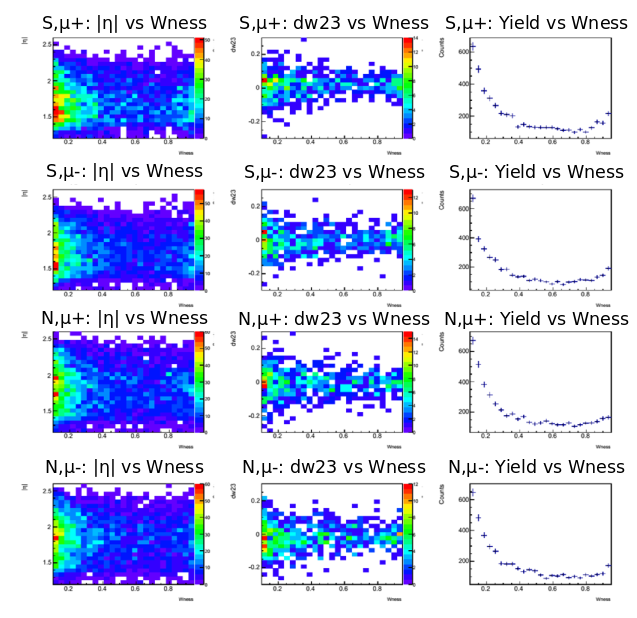
\includegraphics[width=\linewidth]{./figures/dw23_vs_wness_data.png}
  \caption{
    The first column of plots is $\eta$ plotted as a function of $W_{ness}$
    where we see a 2D histogram of the even distribution. The middle column is
    $dw_{23}$ as a function of $W_{ness}$, and the right column is a simple
    histogram of $W_{ness}$. The rows all correspond to the same arm and charge.
    From top to bottom: North, $\mu+$, North $\mu-$, South $\mu+$, North $\mu-$.
    Distributions shown here are all from the physics data set.
  }
  \label{fig:dw23_eta_wness_dat}
\end{figure}

\begin{figure}
  \centering
  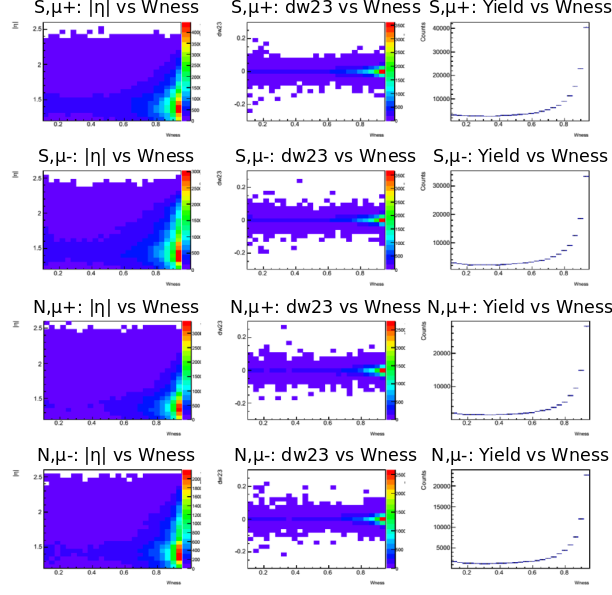
\includegraphics[width=\linewidth]{./figures/dw23_vs_wness_simulation.png}
  \caption{
    The first column of plots is $\eta$ plotted as a function of $W_{ness}$
    where we see a 2D histogram of the even distribution. The middle column is
    $dw_{23}$ as a function of $W_{ness}$, and the right column is a simple
    histogram of $W_{ness}$. The rows all correspond to the same arm and charge.
    From top to bottom: North, $\mu+$, North $\mu-$, South $\mu+$, North $\mu-$.
    Distributions shown here are all from simulated W-genic data set.
  }
  \label{fig:dw23_eta_wness_sim}
\end{figure}

Two features to note from Figure~\ref{fig:dw23_eta_wness_dat} and
Figure~\ref{fig:dw23_eta_wness_sim} is that the distribution for $dw_{23}$
should be expected to be quite narrow for W-genic events, whereas $\eta$ is more
broad. We have good statistic for $\eta$ over all orders of magnitude, so we can
directly construct PDFs for this variable from a binned dataset. However, with
$dw_{23}$ we need to be more careful, as this variable will offer us the
analyzing power.

We create a model for $dw_{23}$, to fully parameterize the event distribution
when viewed as a function of $dw_{23}$ vs $W_{ness}$. We model this by assuming
that the $dw_{23}$ vs $W_{ness}$ distribution can be separated into two parts:

\begin{equation}
  F(W_{ness},dw_{23}) = f(W_{ness})\times g(W_{ness},dw_{23}) 
  \label{eq:dw23_final_parameterization}
\end{equation}

$f(W_{ness})$ is modeled simply as a fourth-degree polynomial (the third column)
of Figures~\ref{fig:dw23_eta_wness_dat} and \ref{fig:dw23_eta_wness_sim}. The
polynomial fit is summarized in Equation~\ref{eq:wness_pol4} and
Figure~\ref{fig:wness_pol4}:

\begin{equation} \label{eq:wness_pol4}
  f(W_{ness}) = 
  P_8 + P_9 W_{ness} + 
  P_{10} {W_{ness}}^2 +
  P_{11} + {W_{ness}}^3 +
  P_{12} + {W_{ness}}^4
\end{equation}

\begin{figure}
  \centering
  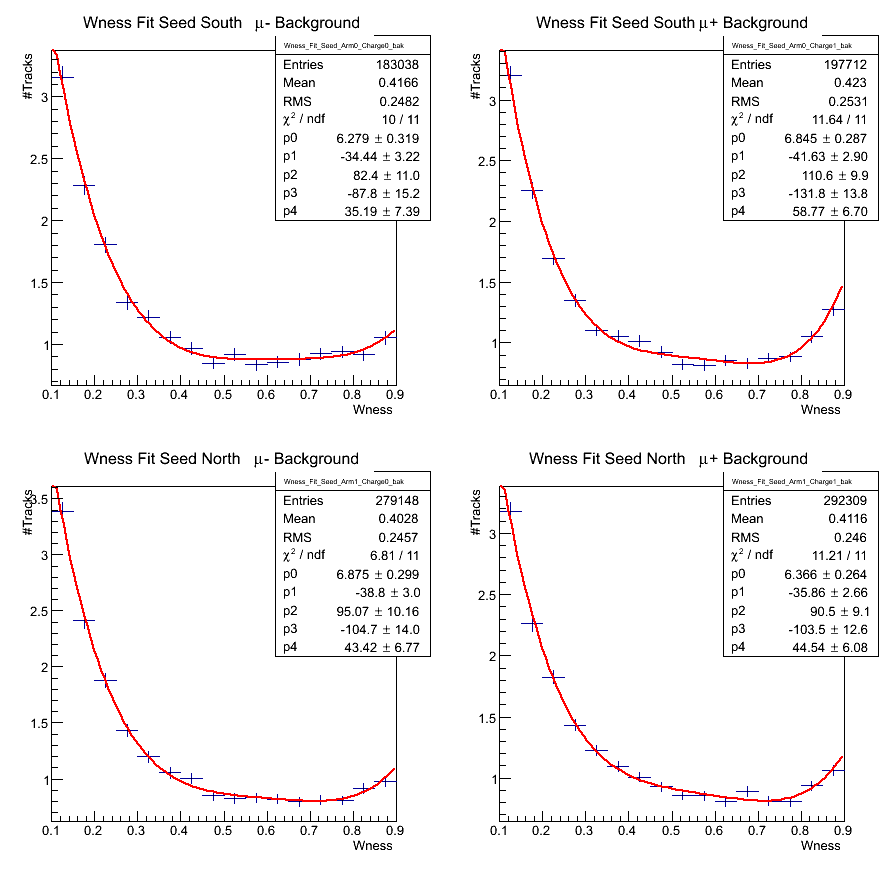
\includegraphics[width=0.7\linewidth]{./figures/c_WnessFit1D.png}
  \caption{
    A summary of the fourth degree polynomial fit (Equation~\ref{eq:wness_pol4})
    to the $W_{ness}$ distribution from the physics dataset in the background
    region.
  }

  \label{fig:wness_pol4}
\end{figure}

We then model the other element of the distribution $g(W_{ness},dw_{23}$ as a
co-axial double Gaussian. We allow the Parameters of the co-axial double
Gaussian to vary linearly with $W_{ness}$, as seen below:

\begin{align}\label{eq_dw23_equations}
  \sigma_1 &= P_1 + P_3 \times W_{ness} &  C_g &= P_6 + P_7 \times W_{ness} \\
  \sigma_2 &= P_4 + P_5 \times W_{ness} &  \mu &= P_0 + P_1 \times W_{ness}
\end{align}

\begin{equation}
  g(W_{ness},dw_{23}) = C_w \times 
  \left(
    \left( 
      { {1}\over{\sqrt{2\pi}\sigma_1+C_g\sqrt{2\pi}\sigma_2} }
    \right) 
    \times
    \left(
      e^{{{1}\over{2}}{\left({dw_{23-\mu}}\over{\sigma_1}\right)^2}}
        +C_ge^{{{1}\over{2}}{\left({dw_{23-\mu}}\over{\sigma_2}\right)^2}} 
    \right) 
  \right)
  \label{eq:dw23_parameterization}
\end{equation}

We seed these linearized parameters by taking slices of $dw_{23}$ in $W_{ness}$
and then fitting this slice with a co-axial double Gaussian. The parameters of
the results of these fits are then plotted against the value of the $W_{ness}$
slice, and fit with a line. These parameters are then used to seed the fit of
Equation~\ref{eq:dw23_final_parameterization} to the physics data set. Fits to
the individual slices of $dw_{23}$ are summarized in
Figure~\ref{fig:dw23_slice_fits}. The results of the co-axial double Gaussian
parameters as functions of $W_{ness}$ slice are shown in
Figure~\ref{fig:coax_params_vs_wness}.

\begin{figure}
  \centering
  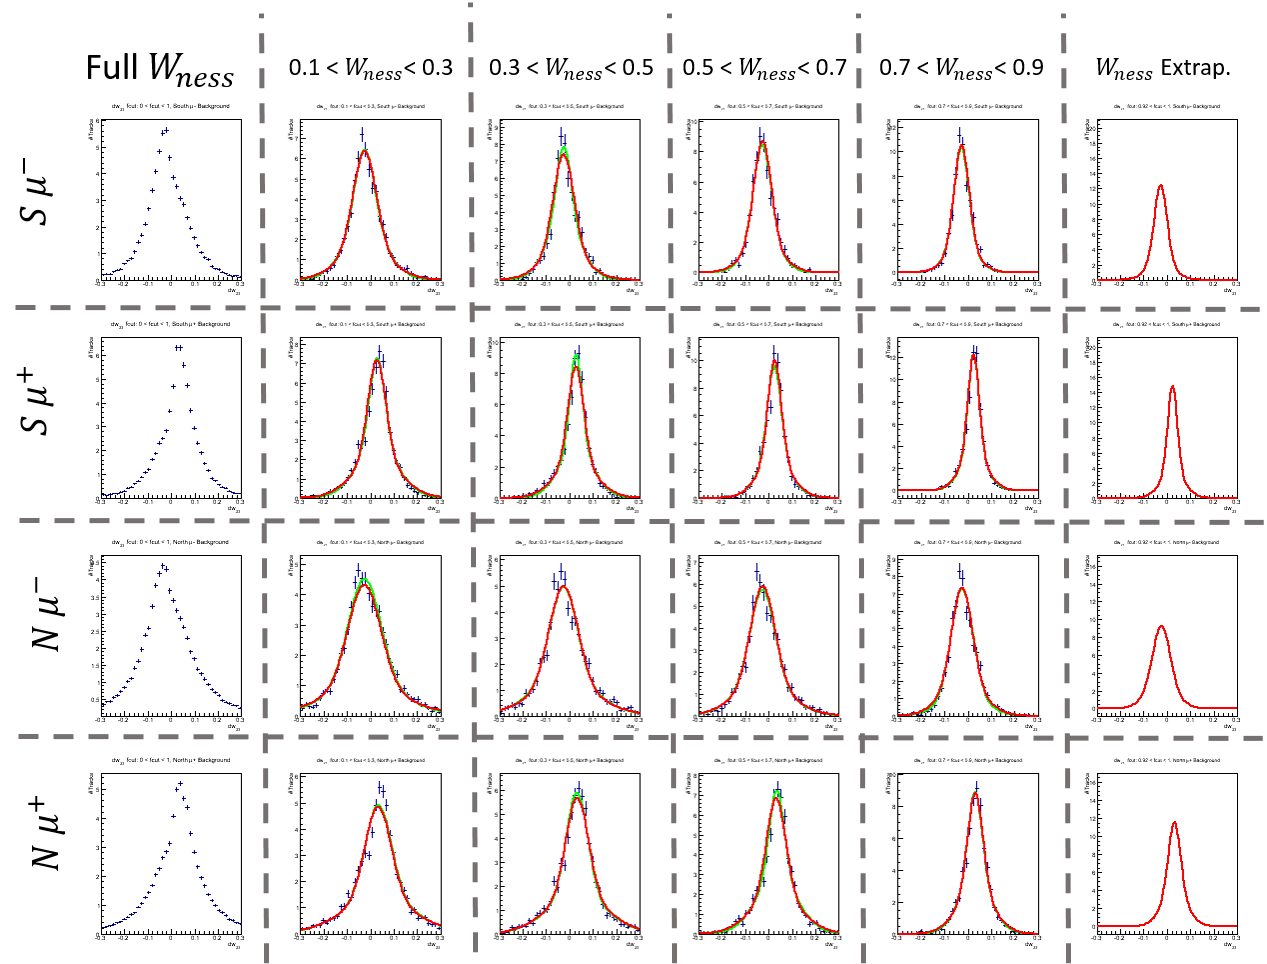
\includegraphics[width=\linewidth]{./figures/dw23_extrap_bins.png}
  \caption{
    From left to right the columns are: $dw_{23}$ for the full $W_{ness}$ range,
    $0.1 < W_{ness} < 0.3$, $0.3 < W_{ness} < 0.7$, $0.3 < W_{ness} < 0.7$, 
    $0.7 < W_{ness} < 0.9$, and finally the extrapolated shape for $W_{ness} >
    0.95$. In red, we see the 1D projection of the 2D distribution to the slice.
    This overlays a green curve, which is a fit done independently to a slice.
    The rows are labeled with the Arm and charge corresponding to the subdivided
    dataset. As you can see, the matching is often exact, between green and red
    curves. As the final column is the extrapolation, there is no slice-fit.
  }
  \label{fig:dw23_slice_fits}
\end{figure}

\begin{figure}
  \centering
  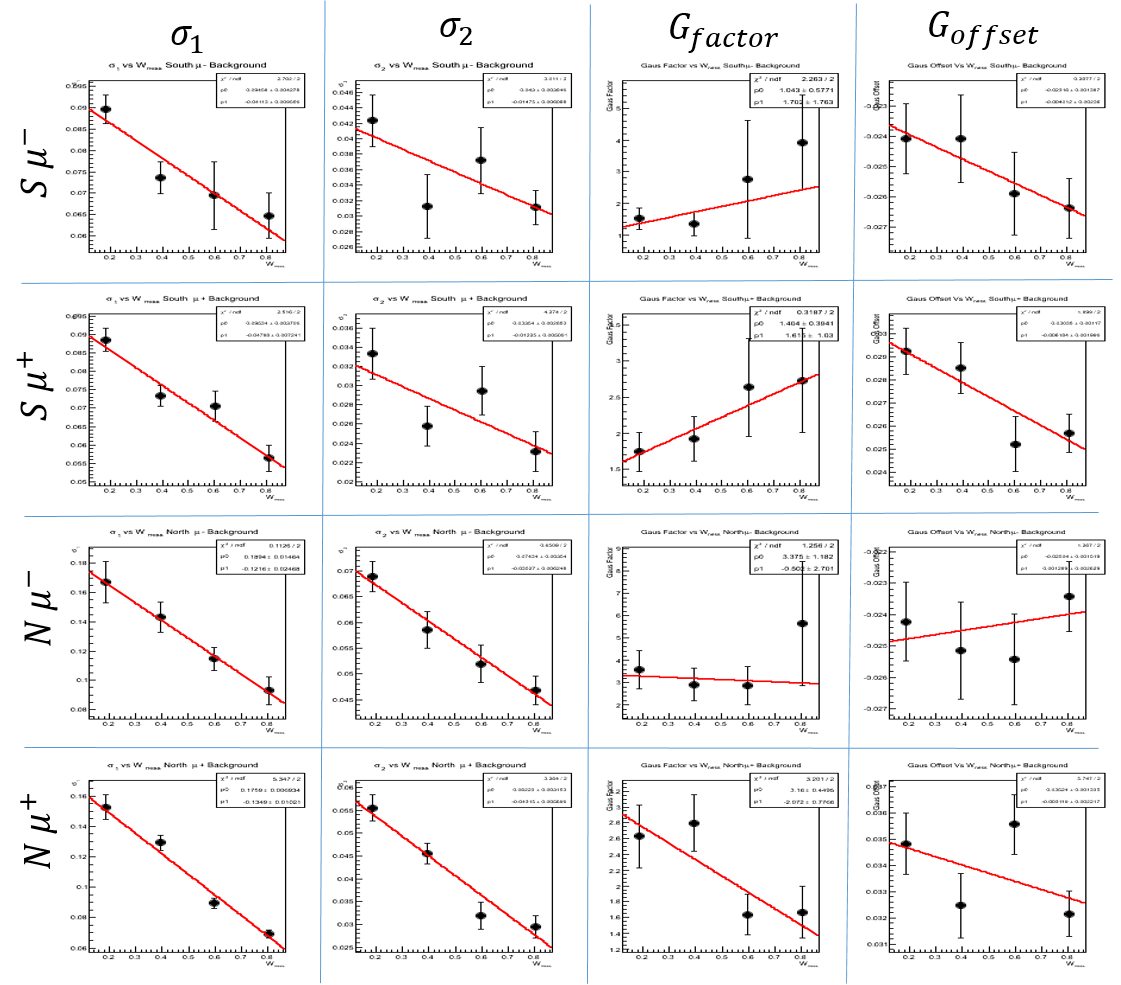
\includegraphics[width=\linewidth]{./figures/dw23_parameters_linearized.png}
  \caption{
    The four parameters from the co-axial Gaussian parameterization of $dw_{23}$
    as a function of $W_{ness}$. Though some parameters ($G_{factor}$, $N\mu-$)
    may appear to be non-linear, note that the uncertainty on some bins is quite
    large. Rows are arm/charge, labeled on the left, while columns are co-axial
    Gaussian parameters, summarized in Equation~\ref{eq:dw23_parameterization}
  }
  \label{fig:coax_params_vs_wness}
\end{figure}

The results of this fitting procedure are summarized in
Figure~\ref{fig:dw23_fits}.

\begin{figure}
  \centering
	\begin{subfigure}[t]{0.5\textwidth}
		\centering
    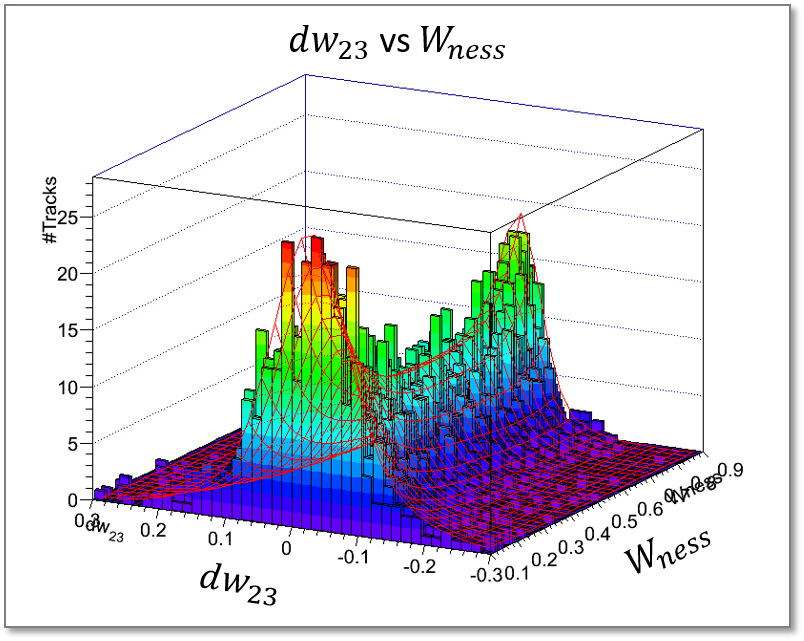
\includegraphics[width=0.95\linewidth]{./figures/dw23_vs_eta_3D.png}
    \caption{The final fit to $dw_{23}$ vs $W_{ness}$}
		\label{fig:3Ddw23_wness}
	\end{subfigure}%
  \begin{subfigure}[t]{0.5\textwidth}
		\centering
		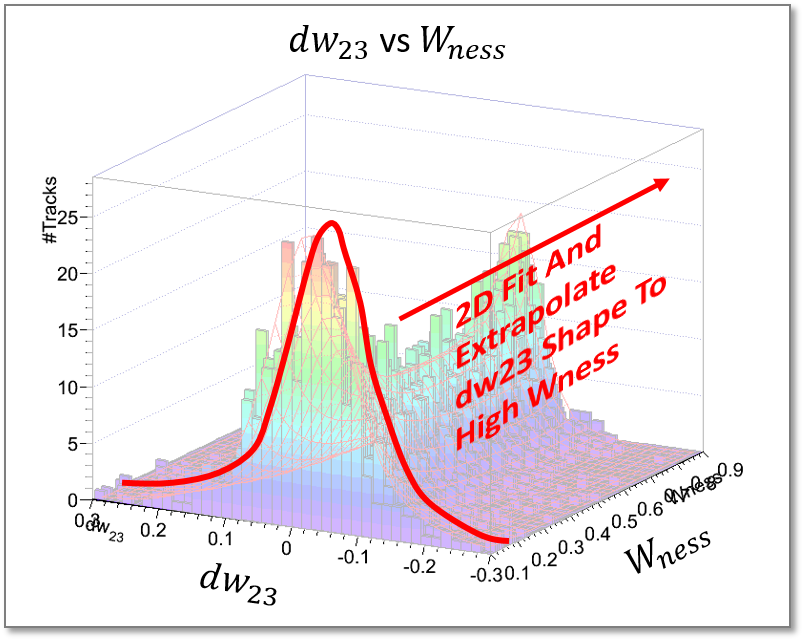
\includegraphics[width=0.95\linewidth]{./figures/dw23_vs_eta_3D_overlay.png}
    \caption{Cartoon of the extrapolation}
		\label{fig:3Ddw23_wness_overlay}
	\end{subfigure}
  \caption{
    The red wire-frame is the resultant fit of to the $dw_{23}$ vs $W_{ness}$
    distribution. We extrapolate the shape of $dw_{23}$ to the signal region to
    obtain the hadronic background PDF for $dw_{23}$.
  }
  \label{fig:dw23_fits}
\end{figure}

\begin{figure}
  \centering
  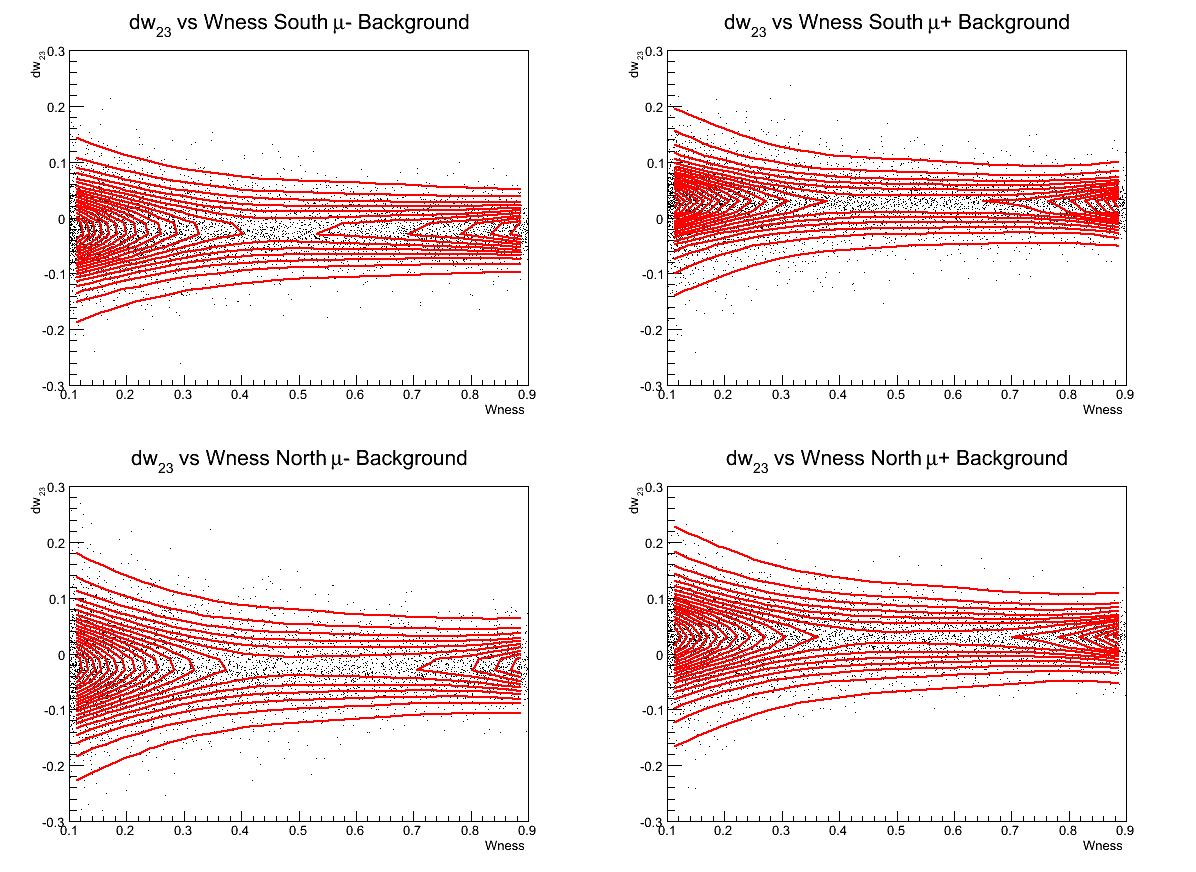
\includegraphics[width=\linewidth]{./figures/c_WnessVsdw23.png}
  \caption{
    An overhead view of the various results of the $dw_{23}$ vs $W_{ness}$ fit
    for each arm and charge combination.
  }
\end{figure}

Finally, the extrapolation of $dw_{23}$ was reproduced independently by four
separate analyzers, Daniel, Abraham, Ralf and Myself, with distributions lining
up very closely, Figure~\ref{fig:four_dw23}

\begin{figure}
  \centering
  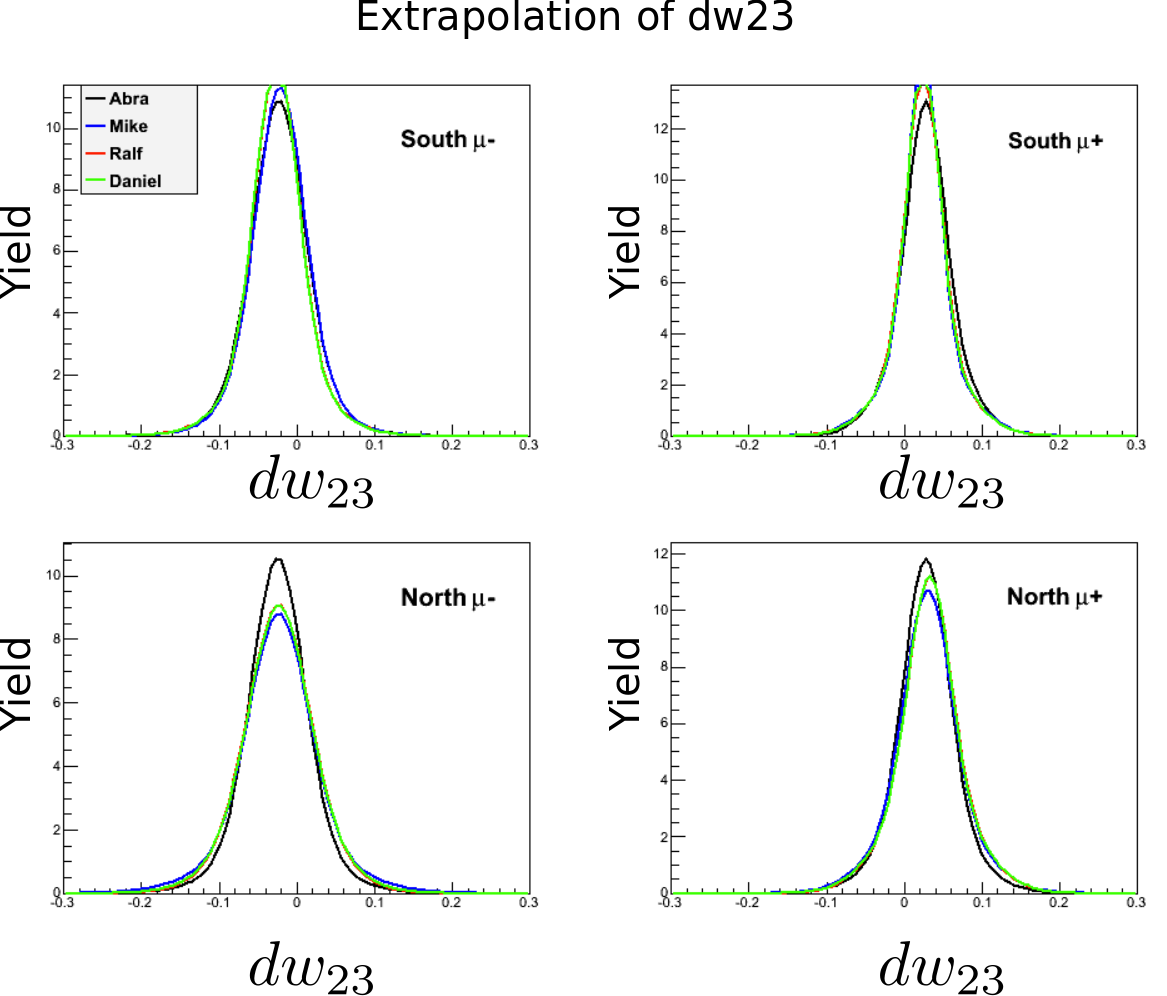
\includegraphics[width=0.7\linewidth]{./figures/dw23_fourway.png}
  \caption{
    Abraham, \textcolor{blue}{Mike}, \textcolor{red}{Ralf} and
    \textcolor{green}{Daniel} all independently parameterized and extrapolated
    $dw_{23}$ obtaining consistent results. Figure prepared by Dr. Francesca
    Giordano~\cite{Seidl2014a}
  }
  \label{fig:four_dw23}
\end{figure}

The PDF for $\eta$ was obtained by creating a histogram of the variable for
events tagged with $W_{ness} < 0.9$. 

\clearpage
\subsection{Muon Background and W-Signal PDFs}

The muon background probability density functions and the W-Signal probability
density functions must be carefully summed from simulations so as to match the
likely composition of the data set. This is done by using the well known
cross-section of each of the processes which are simulated and normalizing with
the integrated luminosity delivered to PHENIX during the 2013 run of RHIC. This
luminosity was found to be $277 pb^{-1}$.

One caveat is that the minimum bias trigger of PHENIX is easily fooled by
effects such as pile-up and multiple collisions. Concretely, this occurs when
there is more than one collision in a single bunch crossing. This is typically
not a problem when PHENIX operates at lower energies and beam luminosities, but
for this data set, it was a real factor, that must be corrected for, else all
the ingredients in the muon background cocktail will be present in the wrong
amounts and we'll get the wrong answer from using them. Pile up refers to the
process where some events aren't read out quickly enough, and so one recorded
event will contain information for two actual beam crossings. Unaccounted for,
pile-up and multiple collisions both have the affect of lowering the measured
luminosity.

The $277 pb^{-1}$ luminosity figure has been corrected for pile-up and multiple
collisions. This is a separate analysis, done by my colleagues working on this
analysis, so it will not be described in detail in this thesis, however it is
described in detail in our analysis note:~\cite{Seidl2014a}.

Finally, the PDFs used in the EULMF are shown in
Figures~\ref{fig:c_dw23_Eta_PDF_Arm0_Charge0}-\ref{fig:c_dw23_Eta_PDF_Arm1_Charge1}.

\begin{figure}
  \centering
  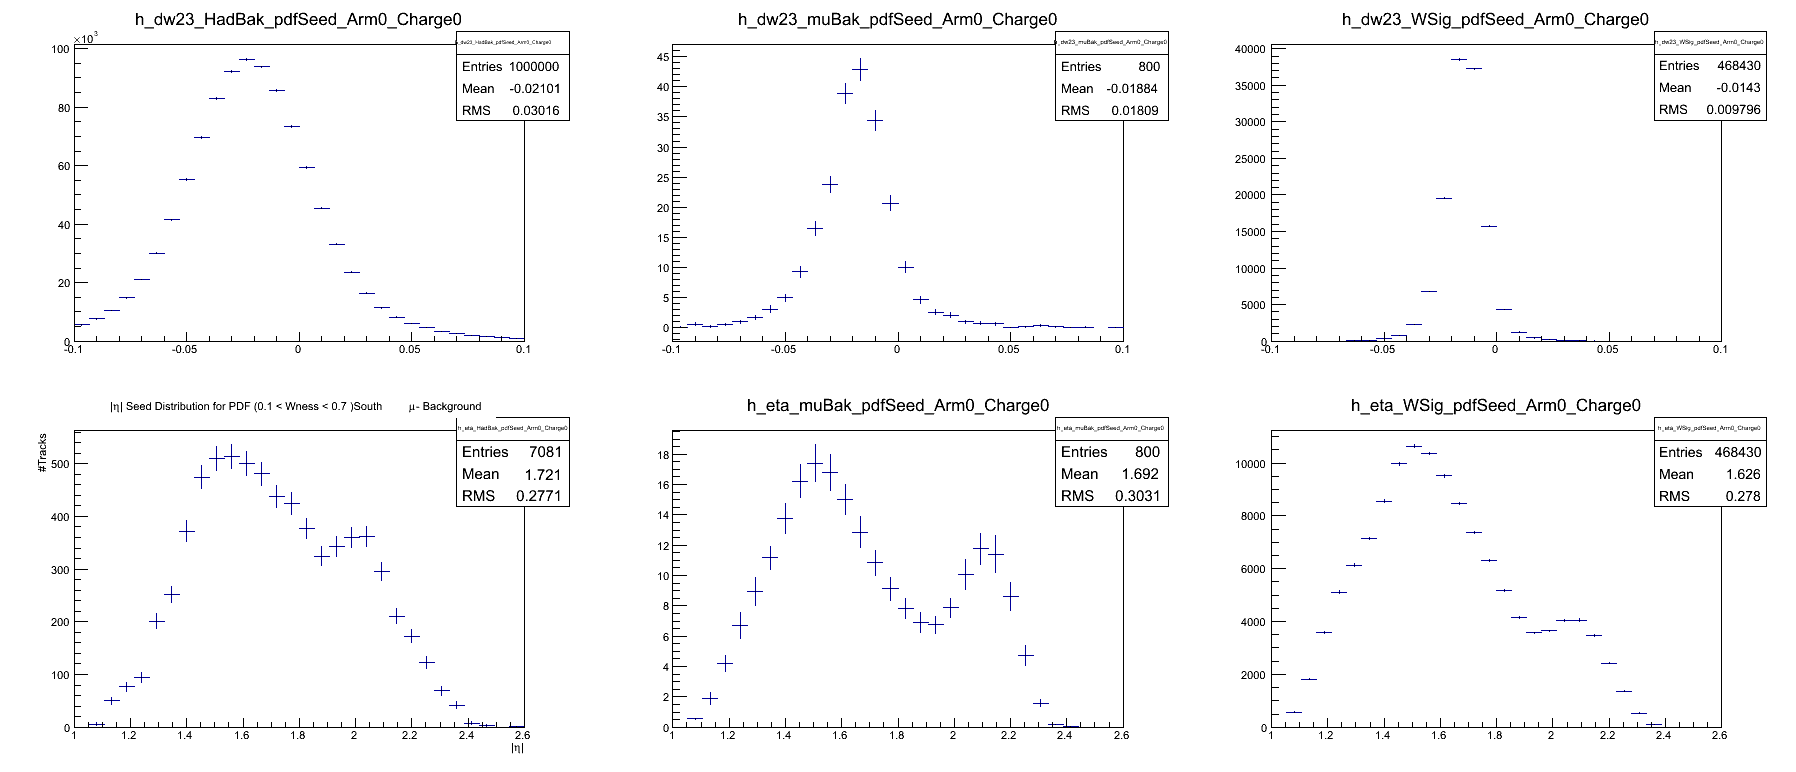
\includegraphics[width=\linewidth]{././figures/c_dw23_Eta_PDF_Arm0_Charge0.png}
  \caption{
    Left Column: The hadronic background PDFs, Middle Column: The Summed Muon
    Background PDFs, Right Column: The W-Signal PDF. For South Arm, $mu+$
  }
  \label{fig:c_dw23_Eta_PDF_Arm0_Charge0}
\end{figure}

\begin{figure}
  \centering
  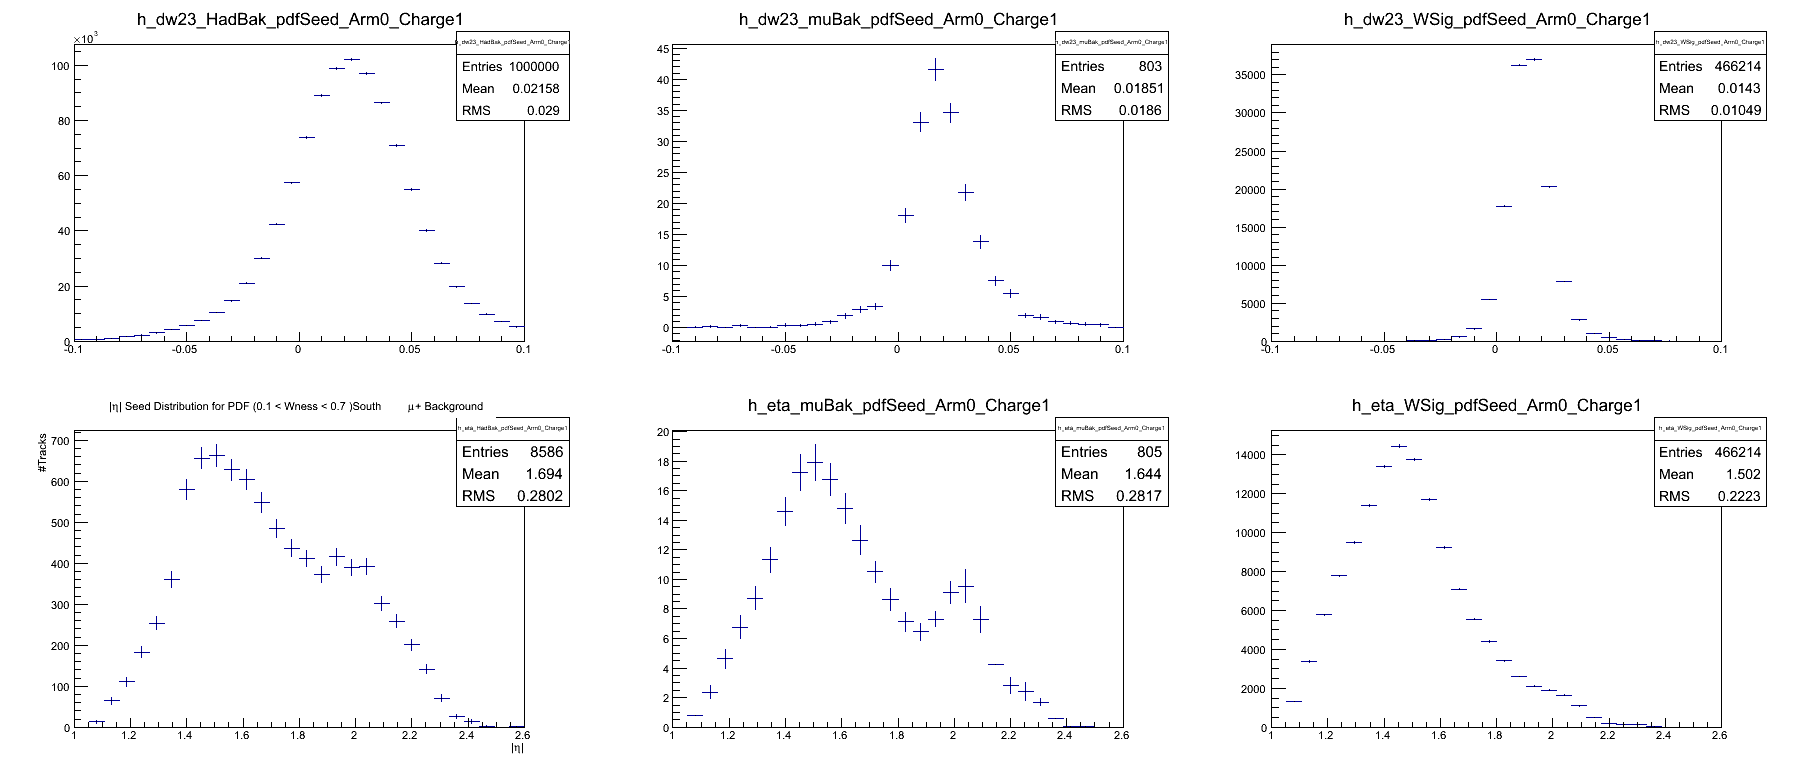
\includegraphics[width=\linewidth]{././figures/c_dw23_Eta_PDF_Arm0_Charge1.png}
  \caption{
    Left Column: The hadronic background PDFs, Middle Column: The Summed Muon
    Background PDFs, Right Column: The W-Signal PDF. For South Arm, $mu-$
  }
  \label{fig:c_dw23_Eta_PDF_Arm0_Charge1}
\end{figure}

\begin{figure}
  \centering
  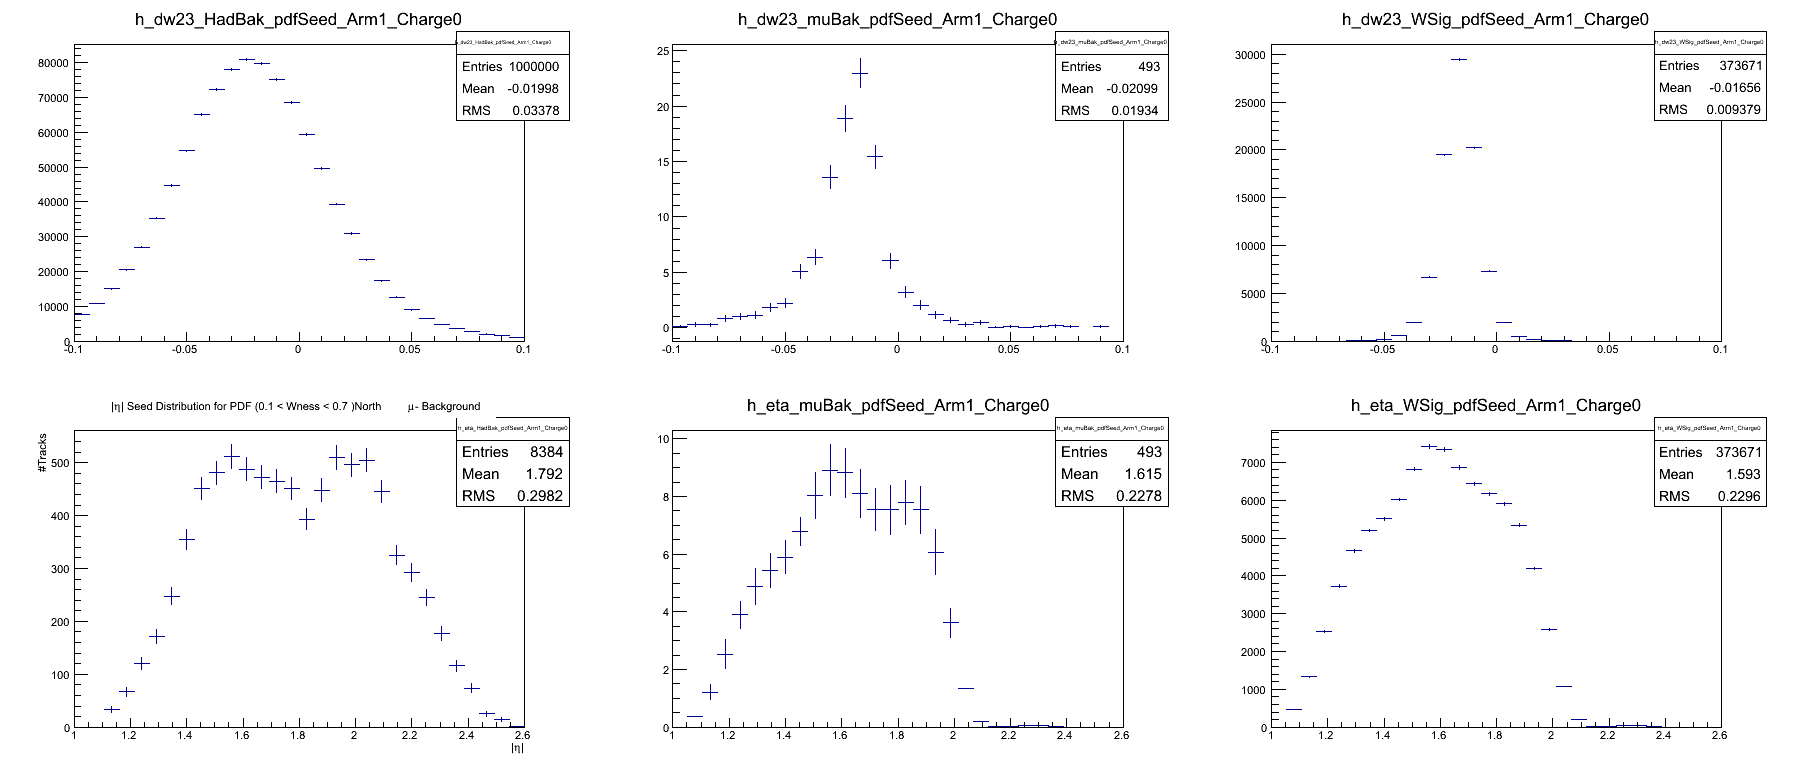
\includegraphics[width=\linewidth]{././figures/c_dw23_Eta_PDF_Arm1_Charge0.png}
  \caption{
    Left Column: The hadronic background PDFs, Middle Column: The Summed Muon
    Background PDFs, Right Column: The W-Signal PDF. For North Arm, $mu-$
  }
  \label{fig:c_dw23_Eta_PDF_Arm1_Charge0}
\end{figure}

\begin{figure}
  \centering
  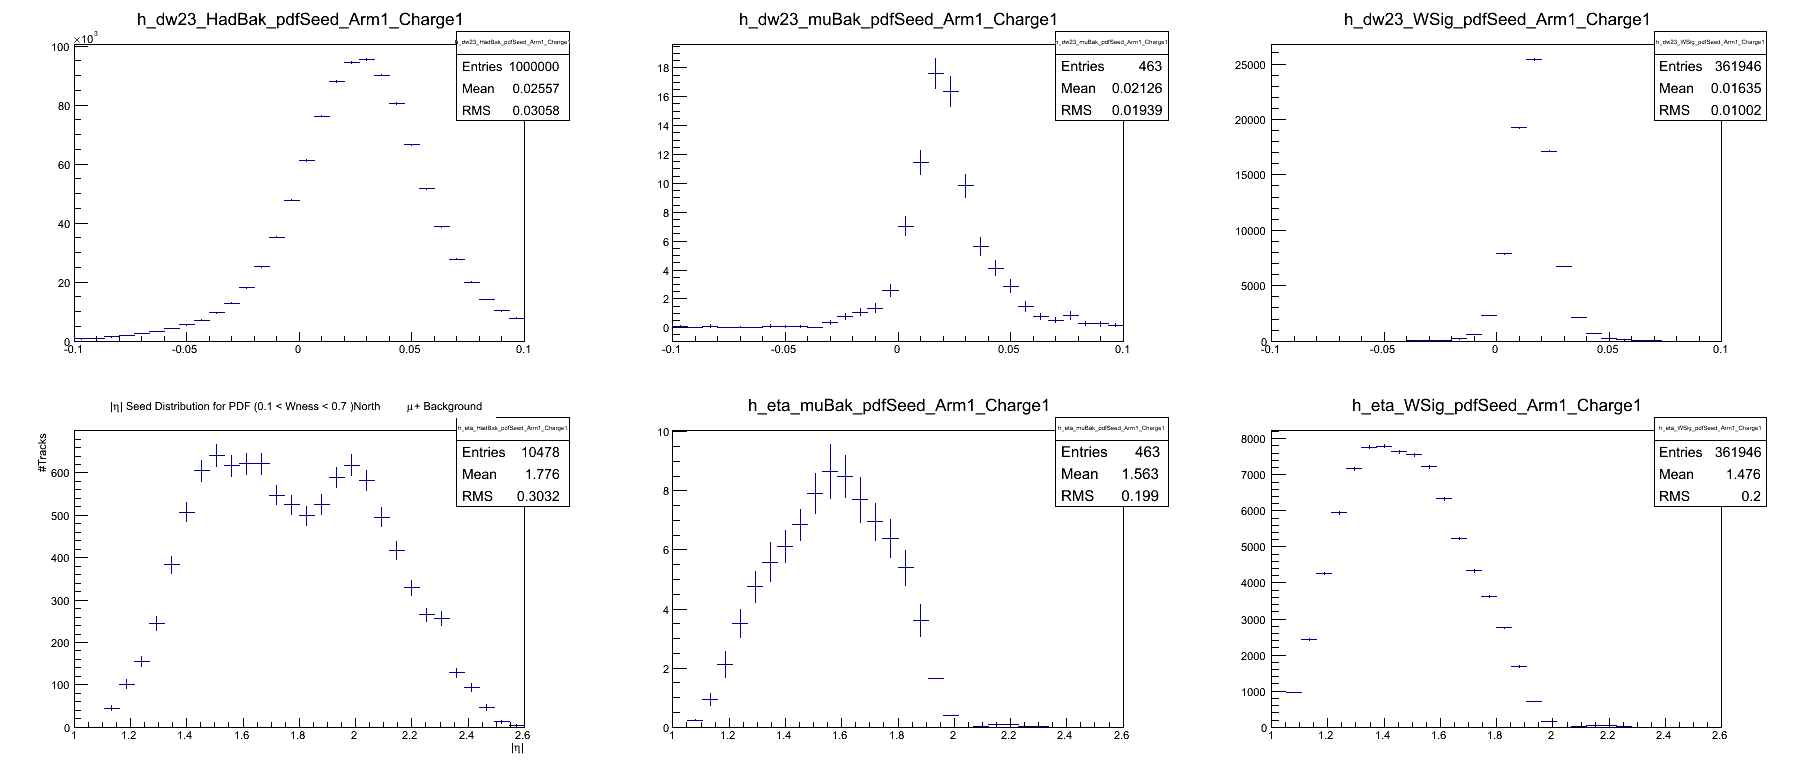
\includegraphics[width=\linewidth]{././figures/c_dw23_Eta_PDF_Arm1_Charge1.png}
  \caption{
    Left Column: The hadronic background PDFs, Middle Column: The Summed Muon
    Background PDFs, Right Column: The W-Signal PDF. For South Arm, $mu+$
  }
  \label{fig:c_dw23_Eta_PDF_Arm1_Charge1}
\end{figure}

With all PDFs prepared, we can perform the extended unbinned maximum likelihood
fit, and extract the yields for the number of signal muons, and the number of
fake hadronic background muons (recalling that the number of muon background
muons are fixed).

\begin{figure}
  \centering
  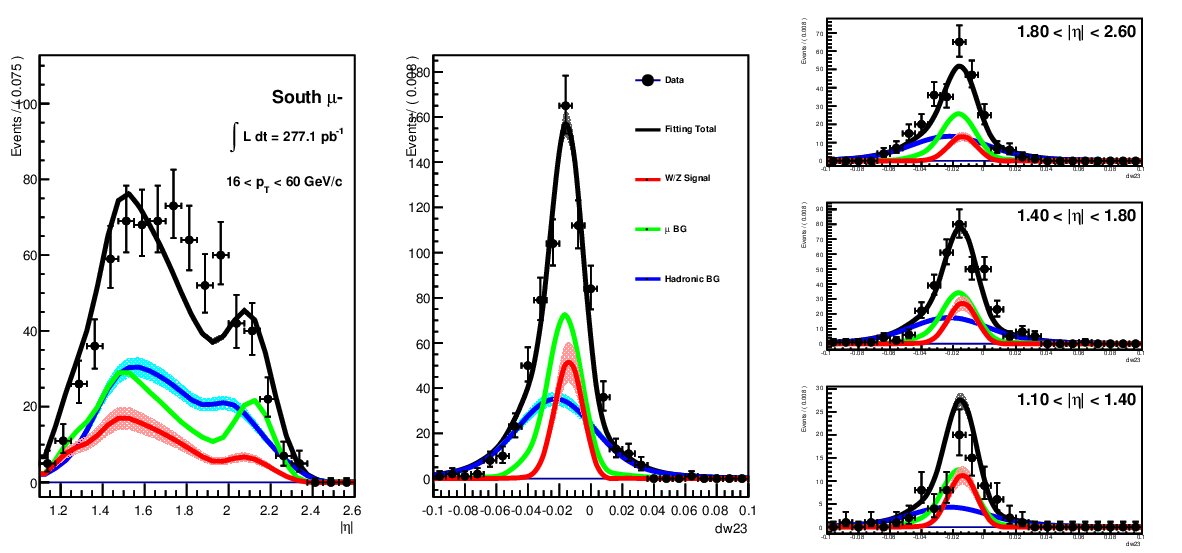
\includegraphics[width=\linewidth]{./figures/prelim_full_maxlikefit_a0q0.jpg}
  \caption{
    Here, we see the preliminary results of the EULMF for the 2013 Run. On the
    left, $\eta$ is shown. In the middle, $dw_{23}$. On the right, $dw_{23}$ is
    subdivided into the three standard $\eta$ bins. In all cases, we see the
    unbinned data in black (with error bars), and the sum of the three fits in
    black. In Blue, we can see the fake-muon hadronic background. In Green, the
    muon background. In blue, we see the W-Signal result. The area under the
    curves represents the yield, relative to the total. Figure prepared by Dr.
    Ralf Seidl~\cite{Seidl2014a}. Shown: South Arm, $\mu-$
  }
  \label{fig:maxlikefit_a0q0}
\end{figure}

\begin{figure}
  \centering
  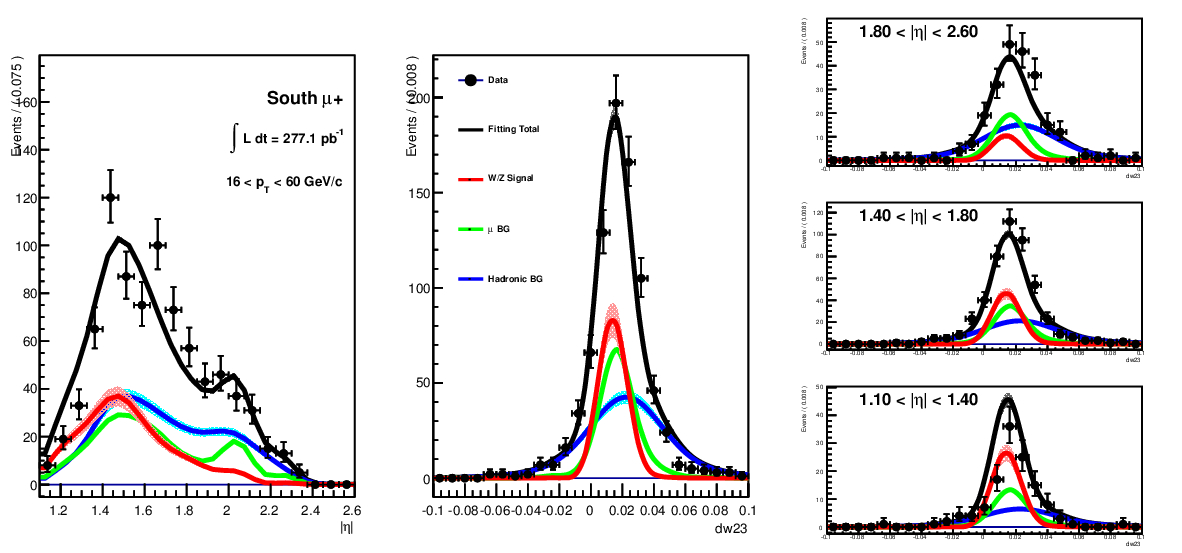
\includegraphics[width=\linewidth]{./figures/prelim_full_maxlikefit_a0q1.jpg}
  \caption{
    Here, we see the preliminary results of the EULMF for the 2013 Run. On the
    left, $\eta$ is shown. In the middle, $dw_{23}$. On the right, $dw_{23}$ is
    subdivided into the three standard $\eta$ bins. In all cases, we see the
    unbinned data in black (with error bars), and the sum of the three fits in
    black. In Blue, we can see the fake-muon hadronic background. In Green, the
    muon background. In blue, we see the W-Signal result. The area under the
    curves represents the yield, relative to the total. Figure prepared by Dr.
    Ralf Seidl~\cite{Seidl2014a}. Shown: South Arm, $\mu+$
  }
  \label{fig:maxlikefit_a0q1}
\end{figure}

\begin{figure}
  \centering
  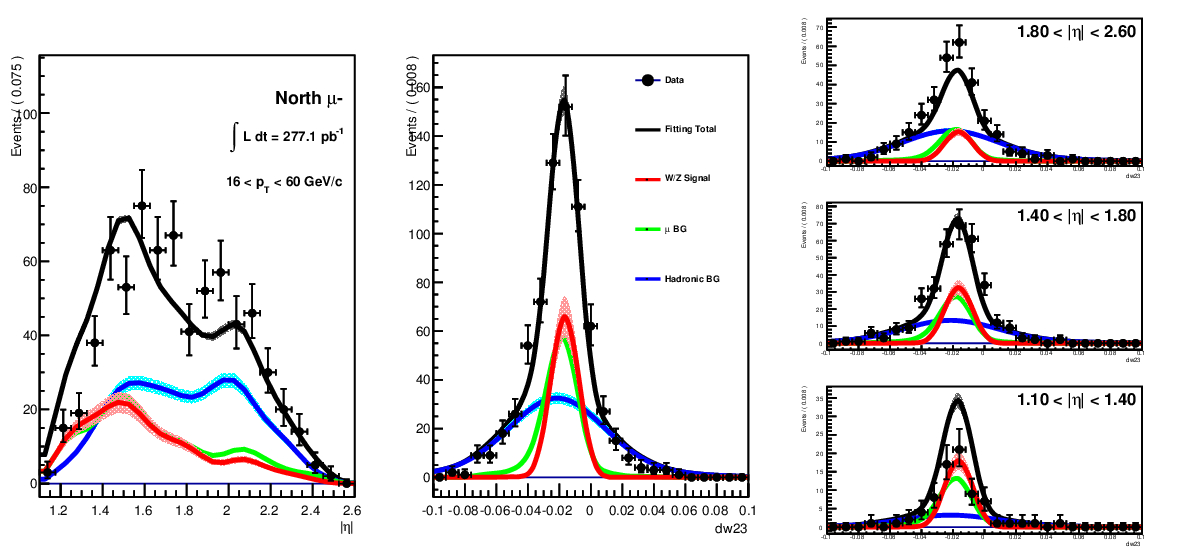
\includegraphics[width=\linewidth]{./figures/prelim_full_maxlikefit_a1q0.jpg}
  \caption{
    Here, we see the preliminary results of the EULMF for the 2013 Run. On the
    left, $\eta$ is shown. In the middle, $dw_{23}$. On the right, $dw_{23}$ is
    subdivided into the three standard $\eta$ bins. In all cases, we see the
    unbinned data in black (with error bars), and the sum of the three fits in
    black. In Blue, we can see the fake-muon hadronic background. In Green, the
    muon background. In blue, we see the W-Signal result. The area under the
    curves represents the yield, relative to the total. Figure prepared by Dr.
    Ralf Seidl~\cite{Seidl2014a}. Shown: North Arm, $\mu-$
  }
  \label{fig:maxlikefit_a1q0}
\end{figure}

\begin{figure}
  \centering
  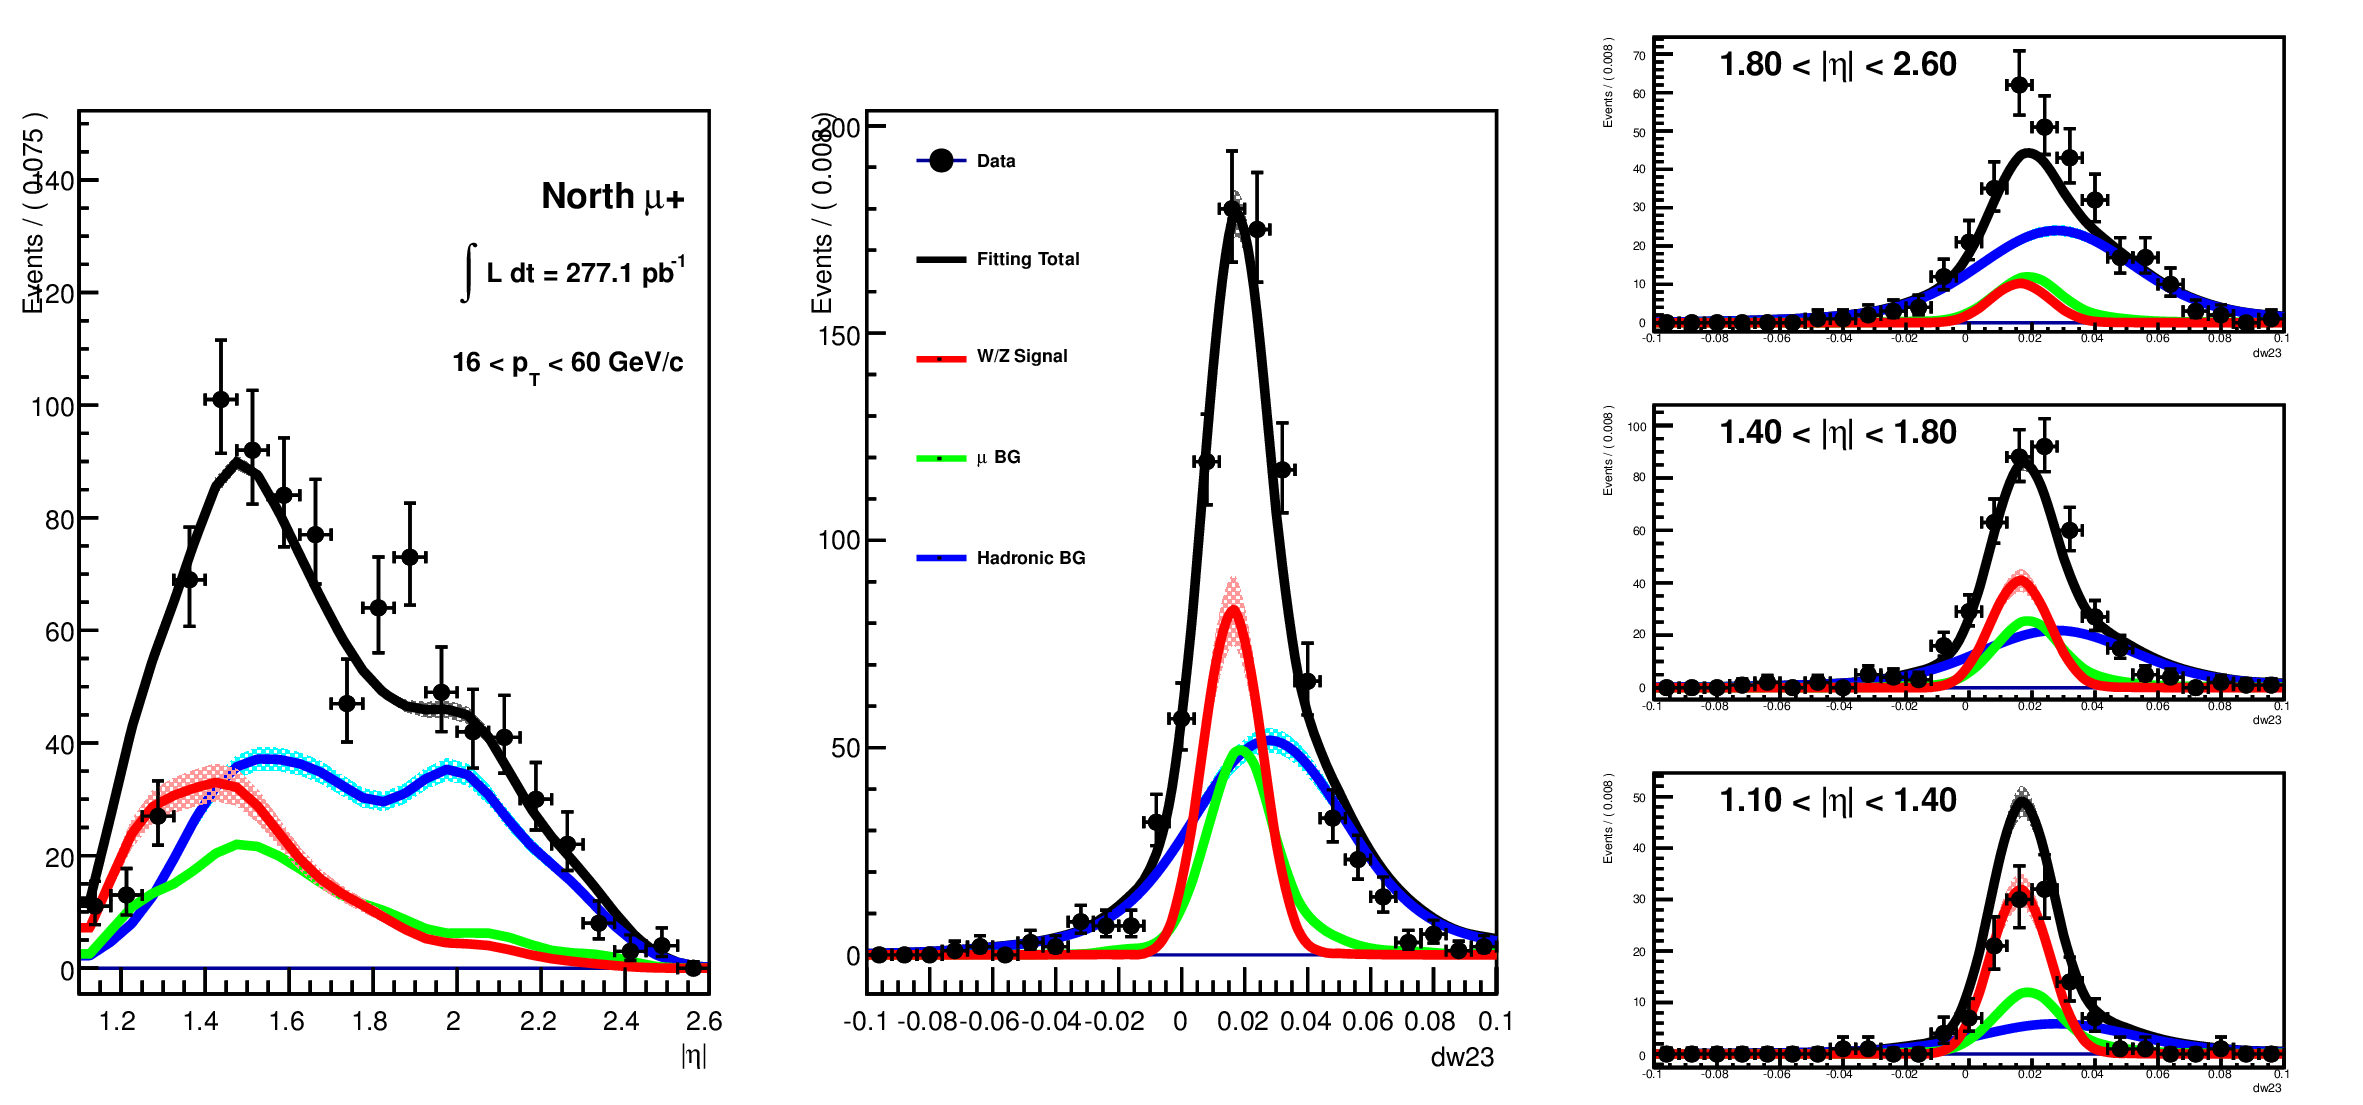
\includegraphics[width=\linewidth]{./figures/prelim_full_maxlikefit_a1q1.jpg}
  \caption{
    Here, we see the preliminary results of the EULMF for the 2013 Run. On the
    left, $\eta$ is shown. In the middle, $dw_{23}$. On the right, $dw_{23}$ is
    subdivided into the three standard $\eta$ bins. In all cases, we see the
    unbinned data in black (with error bars), and the sum of the three fits in
    black. In Blue, we can see the fake-muon hadronic background. In Green, the
    muon background. In blue, we see the W-Signal result. The area under the
    curves represents the yield, relative to the total. Figure prepared by Dr.
    Ralf Seidl~\cite{Seidl2014a}. Shown: North Arm, $\mu+$
  }
  \label{fig:maxlikefit_a1q1}
\end{figure}

The signal to background ratio extraction is summarized by each analyzer in
Table~\ref{tab:sbr_per_analyzer}, for the South Arm $\mu-$ (the canonical
cross check).

\begin{table}[h]
  \centering
  \resizebox{\textwidth}{!}{\begin{tabular}{c|rrrr}
    \toprule
    \multicolumn{5}{c}{\textbf{South $\mu ^{-}$}}  \\  
    \textbf{Variable} & \textbf{Ralf} & \textbf{Daniel} & \textbf{Mike} &
    \textbf{Abraham} \\  
    \midrule
    \textbf{Total events} & $    2032$&$    2034$&$     2022$&$     2039$\\ 
    \textbf{Signal events} & $     340^{+42.14} _{-41.42}$&$      303^{+42.31} _{-41.59}$&$      332^{+42.28} _{-41.58}$&$      294^{+41.38} _{-41.38}$\\ 
    \textbf{Hadron events} & $    1424^{+53.57} _{-52.60}$&$     1469^{+54.55} _{-53.59}$&$     1433^{+53.97} _{-52.99}$&$     1485^{+53.85} _{-53.85}$\\ 
    \textbf{Muon events} & $     269$&$     262$&$      257$&$      259$\\  
    \textbf{Signal/BG} & $    0.20^{+0.03} _{-0.03}$&$     0.18^{+0.00} _{-0.00}$&$     0.20^{+0.03} _{-0.03}$&$     0.17^{+0.02} _{-0.00}$\\ 
    \bottomrule
\end{tabular}}
  \caption{ South arm $W\rightarrow \mu^{-}$ fit results per analyzer
  ~\cite{Seidl2014a}}
  \label{tab:sbr_per_analyzer}
\end{table}
\clearpage

\begin{sidewaystable}
  \centering
  \resizebox{\textwidth}{!}{\begin{tabular}{llccccc}
      \toprule
      \textbf{Arm} & 
      \textbf{Charge} & 
      \textbf{Total Events} & 
      \textbf{Signal Events} & 
      \textbf{Fake Muons} & 
      \textbf{Muon Background} & 
      \textbf{SBR} \\
      \midrule
      S & $\mu-$ & 2023 & $354^{+41.9714}_{-41.2598}$ & $1448^{53.6777}_{-52.7162}$ & $221^{0.212103}_{0.0263482}$ & 0.0258992 \\
      S & $\mu+$ & 2468 & $498^{+44.0941}_{-43.2297}$ & $1767^{57.046 }_{-56.3006}$ & $203^{0.252792}_{0.0238242}$ & 0.0233755 \\
      N & $\mu-$ & 2029 & $370^{+34.4599}_{-33.7046}$ & $1555^{48.5042}_{-47.6586}$ & $104^{0.223026}_{0.0219055}$ & 0.0214353 \\
      N & $\mu+$ & 2633 & $505^{+37.9628}_{-37.2192}$ & $2043^{54.5676}_{-53.7571}$ & $85 ^{0.237312}_{0.0189323}$ & 0.0185715 \\
      \bottomrule
  \end{tabular}}
  \caption{ 
    A summary table from the results of the EULMF to the unbinned data set,
    summed to one $\eta$ bin per arm and charge.
  }
\end{sidewaystable}

\section{Systematic Tests}

One of the rare advantages of this analysis was that I had the opportunity to
undertake it in parallel with others, working as a team to accomplish our goals.
That means that we were able perform many systematic tests. These tests are
summarized in the Appendix~\ref{appendix_1}, and serve to lend confidence to our
extraction of the signal to background ratio.
